% Options for packages loaded elsewhere
\PassOptionsToPackage{unicode}{hyperref}
\PassOptionsToPackage{hyphens}{url}
%
\documentclass[
  6pt,
]{article}
\usepackage{lmodern}
\usepackage{amssymb,amsmath}
\usepackage{ifxetex,ifluatex}
\ifnum 0\ifxetex 1\fi\ifluatex 1\fi=0 % if pdftex
  \usepackage[T1]{fontenc}
  \usepackage[utf8]{inputenc}
  \usepackage{textcomp} % provide euro and other symbols
\else % if luatex or xetex
  \usepackage{unicode-math}
  \defaultfontfeatures{Scale=MatchLowercase}
  \defaultfontfeatures[\rmfamily]{Ligatures=TeX,Scale=1}
\fi
% Use upquote if available, for straight quotes in verbatim environments
\IfFileExists{upquote.sty}{\usepackage{upquote}}{}
\IfFileExists{microtype.sty}{% use microtype if available
  \usepackage[]{microtype}
  \UseMicrotypeSet[protrusion]{basicmath} % disable protrusion for tt fonts
}{}
\makeatletter
\@ifundefined{KOMAClassName}{% if non-KOMA class
  \IfFileExists{parskip.sty}{%
    \usepackage{parskip}
  }{% else
    \setlength{\parindent}{0pt}
    \setlength{\parskip}{6pt plus 2pt minus 1pt}}
}{% if KOMA class
  \KOMAoptions{parskip=half}}
\makeatother
\usepackage{xcolor}
\IfFileExists{xurl.sty}{\usepackage{xurl}}{} % add URL line breaks if available
\IfFileExists{bookmark.sty}{\usepackage{bookmark}}{\usepackage{hyperref}}
\hypersetup{
  pdftitle={Measuring the effect of different political actions to contrast the contagion of COVID19},
  hidelinks,
  pdfcreator={LaTeX via pandoc}}
\urlstyle{same} % disable monospaced font for URLs
\usepackage[margin=1in]{geometry}
\usepackage{longtable,booktabs}
% Correct order of tables after \paragraph or \subparagraph
\usepackage{etoolbox}
\makeatletter
\patchcmd\longtable{\par}{\if@noskipsec\mbox{}\fi\par}{}{}
\makeatother
% Allow footnotes in longtable head/foot
\IfFileExists{footnotehyper.sty}{\usepackage{footnotehyper}}{\usepackage{footnote}}
\makesavenoteenv{longtable}
\usepackage{graphicx}
\makeatletter
\def\maxwidth{\ifdim\Gin@nat@width>\linewidth\linewidth\else\Gin@nat@width\fi}
\def\maxheight{\ifdim\Gin@nat@height>\textheight\textheight\else\Gin@nat@height\fi}
\makeatother
% Scale images if necessary, so that they will not overflow the page
% margins by default, and it is still possible to overwrite the defaults
% using explicit options in \includegraphics[width, height, ...]{}
\setkeys{Gin}{width=\maxwidth,height=\maxheight,keepaspectratio}
% Set default figure placement to htbp
\makeatletter
\def\fps@figure{htbp}
\makeatother
\setlength{\emergencystretch}{3em} % prevent overfull lines
\providecommand{\tightlist}{%
  \setlength{\itemsep}{0pt}\setlength{\parskip}{0pt}}
\setcounter{secnumdepth}{-\maxdimen} % remove section numbering
\usepackage{graphicx, amsmath, bm, gensymb}
\usepackage[T1]{fontenc}
\newlength{\cslhangindent}
\setlength{\cslhangindent}{1.5em}
\newenvironment{cslreferences}%
  {\setlength{\parindent}{0pt}%
  \everypar{\setlength{\hangindent}{\cslhangindent}}\ignorespaces}%
  {\par}

\title{Measuring the effect of different political actions to contrast
the contagion of COVID19}
\usepackage{etoolbox}
\makeatletter
\providecommand{\subtitle}[1]{% add subtitle to \maketitle
  \apptocmd{\@title}{\par {\large #1 \par}}{}{}
}
\makeatother
\subtitle{Angela Andreella, Michele Lambardi, Silvia De Nicolò}
\author{}
\date{\vspace{-2.5em}03th June, 2020}

\begin{document}
\maketitle

{
\setcounter{tocdepth}{2}
\tableofcontents
}
\hypertarget{introduction}{%
\section{Introduction}\label{introduction}}

Since the beginning of the COVID-19 epidemic, policymakers in different
countries have introduced different political action to contrast the
contagion. The containment restrictions span from worldwide curfews,
stay-at-home orders, shelter-in-place orders, shutdowns/lockdowns to
softer measures, and stay-at-home recommendations and including besides
the development of contact tracing strategies and specific testing
policies. The pandemic has resulted in the largest amount of
shutdowns/lockdowns worldwide at the same time in history.

The timing of the different interventions, concerning the spread of the
contagion both at a global and intra-national level, has been very
different from country to country. This situation, in combination with
demographical, economic, health-care-related, and area-specific factors,
has resulted in different contagion patterns across the world.

Therefore, our goal is two-fold. The aim is to measure the effect of the
different political actions by analysing and comparing types of actions
from a global perspective and, at the same time, to benchmark the effect
of the same action in a heterogeneous framework such as the Italian
regional context.

In doing so, some issue arises concerning the identification and
codification of the different measures undertaken by governments, the
analysis related to whether a strategies resemblance can be detected
across countries and the measurement of the effects of containment
policies on contagion. Thus, after an introductory section explaining
data and variables, a second section regards some explanatory analysis
facing the codification of containment policies and the strategies
resembling patterns. The third section deals with the measurement of
policies effect from a global perspective, lastly the forth section
analyze Italian lockdown and regional outcomes. The conclusions are
drawn in the last section.

\hypertarget{data-and-variables}{%
\section{Data and Variables}\label{data-and-variables}}

The data repositories used for this project are \emph{COVID-19 Data
Repository by the Center for Systems Science and Engineering (CSSE) at
Johns Hopkins University}\footnote{\url{https://github.com/CSSEGISandData/COVID-19/tree/master/csse_covid_19_data}}
for contagion data (Dong, Du, and Gardner (2020)), and \emph{Oxford
COVID-19 Government Response Tracker (OxCGRT)}\footnote{\url{https://github.com/OxCGRT/covid-policy-tracker}}
for policies tracking (Thomas et al. (2020)), together with \emph{World
Bank Open Data Repository} for demographic data.

As regards contagion data, we used as main variable the active cases,
defined as the total confirmed cases (cumulative confirmed positive
cases including presumptive positive) minus total deaths minus total
recovered. For further information, see Thomas et al. (2020).

As regards policy variables, the \emph{Oxford COVID-19 Government
Response Tracker (OxCGRT)} collects all the containment policies adopted
by the government worldwide by making available information on 11
indicators of government containment responses of ordinal type. These
indicators measure policies on a simple scale of severity/intensity and
are reported for each day a policy is in place, specifying if they are
``targeted'', applying only to a sub-region of a jurisdiction, or a
specific sector; or ``general'', applying throughout that jurisdiction
or across the economy.

The ordinal containment variables considered are:

\begin{longtable}[]{@{}ll@{}}
\toprule
\begin{minipage}[b]{0.09\columnwidth}\raggedright
\textbf{Name}\strut
\end{minipage} & \begin{minipage}[b]{0.85\columnwidth}\raggedright
\textbf{Category}\strut
\end{minipage}\tabularnewline
\midrule
\endhead
\begin{minipage}[t]{0.09\columnwidth}\raggedright
School closing\strut
\end{minipage} & \begin{minipage}[t]{0.85\columnwidth}\raggedright
0 - No measures 1 - recommend closing 2 - Require closing (only some
levels or categories, eg just high school, or just public schools) 3 -
Require closing all levels\strut
\end{minipage}\tabularnewline
\begin{minipage}[t]{0.09\columnwidth}\raggedright
Workplace closing\strut
\end{minipage} & \begin{minipage}[t]{0.85\columnwidth}\raggedright
0 - No measures 1 - recommend closing (or work from home) 2 - require
closing (or work from home) for some sectors or categories of workers 3
- require closing (or work from home) all-but-essential workplaces
(e.g.~grocery stores, doctors)\strut
\end{minipage}\tabularnewline
\begin{minipage}[t]{0.09\columnwidth}\raggedright
Cancel public events\strut
\end{minipage} & \begin{minipage}[t]{0.85\columnwidth}\raggedright
0 - No measures 1 - Recommend cancelling 2 - Require cancelling\strut
\end{minipage}\tabularnewline
\begin{minipage}[t]{0.09\columnwidth}\raggedright
Restrictions on gatherings\strut
\end{minipage} & \begin{minipage}[t]{0.85\columnwidth}\raggedright
0 - No restrictions 1 - Restrictions on very large gatherings (the limit
is above 1000 people) 2 - Restrictions on gatherings between 101-1000
people 3 - Restrictions on gatherings between 11-100 people 4 -
Restrictions on gatherings of 10 people or less\strut
\end{minipage}\tabularnewline
\begin{minipage}[t]{0.09\columnwidth}\raggedright
Close public transport\strut
\end{minipage} & \begin{minipage}[t]{0.85\columnwidth}\raggedright
0 - No measures 1 - Recommend closing (or significantly reduce
volume/route/means of transport available) 2 - Require closing (or
prohibit most citizens from using it)\strut
\end{minipage}\tabularnewline
\begin{minipage}[t]{0.09\columnwidth}\raggedright
Stay at home requirements\strut
\end{minipage} & \begin{minipage}[t]{0.85\columnwidth}\raggedright
0 - No measures 1 - recommend not leaving house 2 - require not leaving
house with exceptions for daily exercise, grocery shopping, and
`essential' trips 3 - Require not leaving house with minimal exceptions
(e.g.~allowed to leave only once a week, or only one person can leave at
a time, etc.)\strut
\end{minipage}\tabularnewline
\begin{minipage}[t]{0.2\columnwidth}\raggedright
Restrictions on internal movements\strut
\end{minipage} & \begin{minipage}[t]{0.85\columnwidth}\raggedright
0 - No measures 1 - Recommend not to travel between regions/cities 2 -
internal movement restrictions in place\strut
\end{minipage}\tabularnewline
\begin{minipage}[t]{0.09\columnwidth}\raggedright
International travel controls\strut
\end{minipage} & \begin{minipage}[t]{0.85\columnwidth}\raggedright
0 - No measures 1 - Screening 2 - Quarantine arrivals from high-risk
regions 3 - Ban on arrivals from some regions 4 - Ban on all regions or
total border closure\strut
\end{minipage}\tabularnewline
\begin{minipage}[t]{0.09\columnwidth}\raggedright
Public info campaigns\strut
\end{minipage} & \begin{minipage}[t]{0.85\columnwidth}\raggedright
0 -No COVID-19 public information campaign 1 - public officials urging
caution about COVID-19 2 - coordinated public information campaign
(e.g.~across traditional and social media)\strut
\end{minipage}\tabularnewline
\begin{minipage}[t]{0.09\columnwidth}\raggedright
Testing policy\strut
\end{minipage} & \begin{minipage}[t]{0.85\columnwidth}\raggedright
0 - No testing policy 1 - Only those who both (a) have symptoms AND (b)
meet specific criteria (e.g.~key workers, admitted to hospital, came
into contact with a known case, returned from overseas) 2 - testing of
anyone showing COVID-19 symptoms 3 - open public testing (e.g.~drive
through testing available to asymptomatic people)\strut
\end{minipage}\tabularnewline
\begin{minipage}[t]{0.09\columnwidth}\raggedright
Contact Tracing Policy\strut
\end{minipage} & \begin{minipage}[t]{0.85\columnwidth}\raggedright
0 - No contact tracing 1 - Limited contact tracing - not done for all
cases 2 - Comprehensive contact tracing - done for all identified
cases\strut
\end{minipage}\tabularnewline
\bottomrule
\end{longtable}

Lastly, a set of confounders variables has been considered in the
analysis. These can be divided into three main areas:

\begin{enumerate}
\def\labelenumi{\arabic{enumi}.}
\item
  \textbf{Longitudinal economic} variables from Thomas et al. (2020);
\item
  \textbf{Longitudinal health system} variables from Thomas et al.
  (2020);
\item
  \textbf{Fixed demographic/economic/health variables} from the
  \href{https://data.worldbank.org/}{World Bank Open Data}.
\end{enumerate}

\hypertarget{longitudinal-economic-variables}{%
\subsection{Longitudinal economic
Variables}\label{longitudinal-economic-variables}}

We analyze \(4\) economic variables from Thomas et al. (2020):

\begin{longtable}[]{@{}lll@{}}
\toprule
\begin{minipage}[b]{0.18\columnwidth}\raggedright
\textbf{Name}\strut
\end{minipage} & \begin{minipage}[b]{0.2\columnwidth}\raggedright
\textbf{Type}\strut
\end{minipage} & \begin{minipage}[b]{0.69\columnwidth}\raggedright
\hspace{3mm}\textbf{Category}\strut
\end{minipage}\tabularnewline
\midrule
\endhead
\begin{minipage}[t]{0.18\columnwidth}\raggedright
Income Support\strut
\end{minipage} & \begin{minipage}[t]{0.04\columnwidth}\raggedright
Ordinal\strut
\end{minipage} & \begin{minipage}[t]{0.69\columnwidth}\raggedright
0 - no income support; 1 - government replaces $<50\%$ of lost salary, 2 - \hspace{5mm} government replaces $>50\%$ of lost
salary\strut
\end{minipage}\tabularnewline
\begin{minipage}[t]{0.18\columnwidth}\raggedright
Debt/contract relief for households\strut
\end{minipage} & \begin{minipage}[t]{0.04\columnwidth}\raggedright
Ordinal \hspace{2mm}\strut
\end{minipage} & \begin{minipage}[t]{0.69\columnwidth}\raggedright
0 - No; 1 - Narrow relief; 2-broad debt/contract relief\strut
\end{minipage}\tabularnewline
\begin{minipage}[t]{0.18\columnwidth}\raggedright
Fiscal measures\strut
\end{minipage} & \begin{minipage}[t]{0.04\columnwidth}\raggedright
USD\hspace{2mm}\strut
\end{minipage} & \begin{minipage}[t]{0.69\columnwidth}\raggedright
\strut
\end{minipage}\tabularnewline
\begin{minipage}[t]{0.18\columnwidth}\raggedright
International support\strut
\end{minipage} & \begin{minipage}[t]{0.04\columnwidth}\raggedright
USD\hspace{2mm}\strut
\end{minipage} & \begin{minipage}[t]{0.69\columnwidth}\raggedright
\strut
\end{minipage}\tabularnewline
\bottomrule
\end{longtable}

However, having \(9\) ordinal policies lockdown covariates, the two
first economic variables are combined into one continuous variable using
the Polychoric Principal Component Analysis, to diminish the number of
covariates inside the model.
\begin{center}
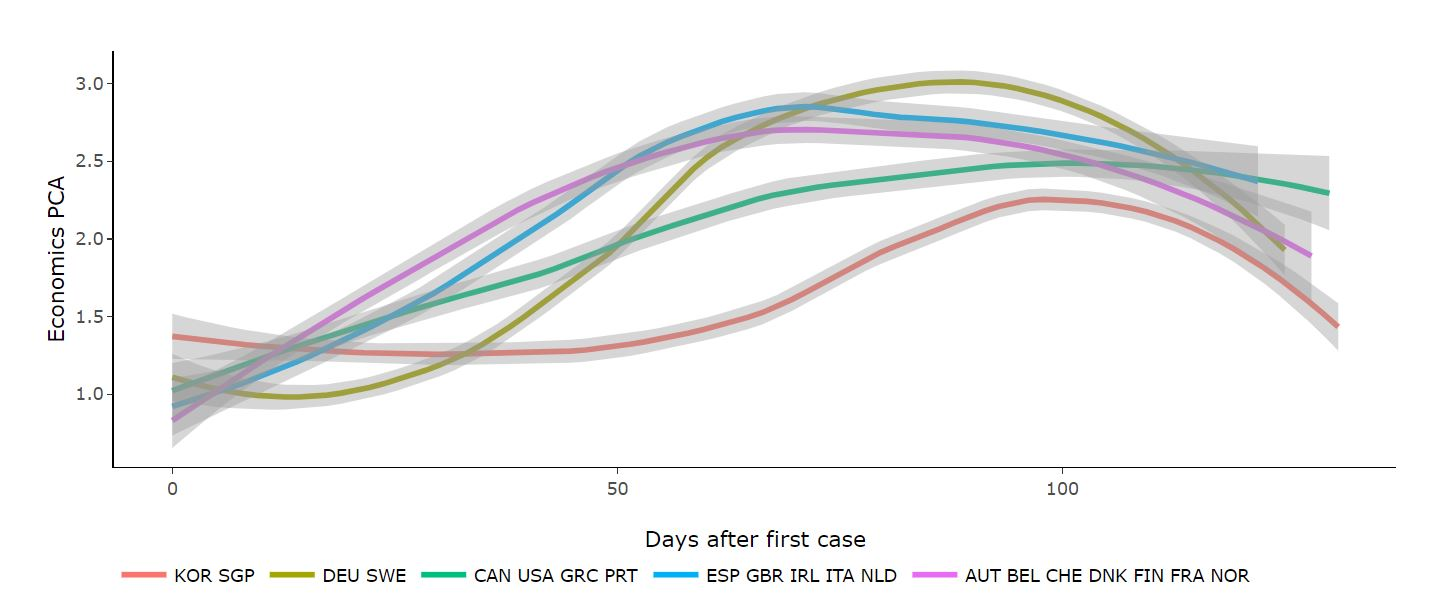
\includegraphics[width=\textwidth]{Report_SC_Group3_files/figure-latex/fig1.jpg}
\end{center}
The Economic PCA has a temporal pattern, with more considerable
variability near the last days of observations. Korea and Singapore's
population received less money from the government than the other
countries. The European ones are the best as financial support to
society.

Therefore, the USD's two economic variables are examined and transformed
into a logarithmic scale to de-emphasize large values.
\begin{center}
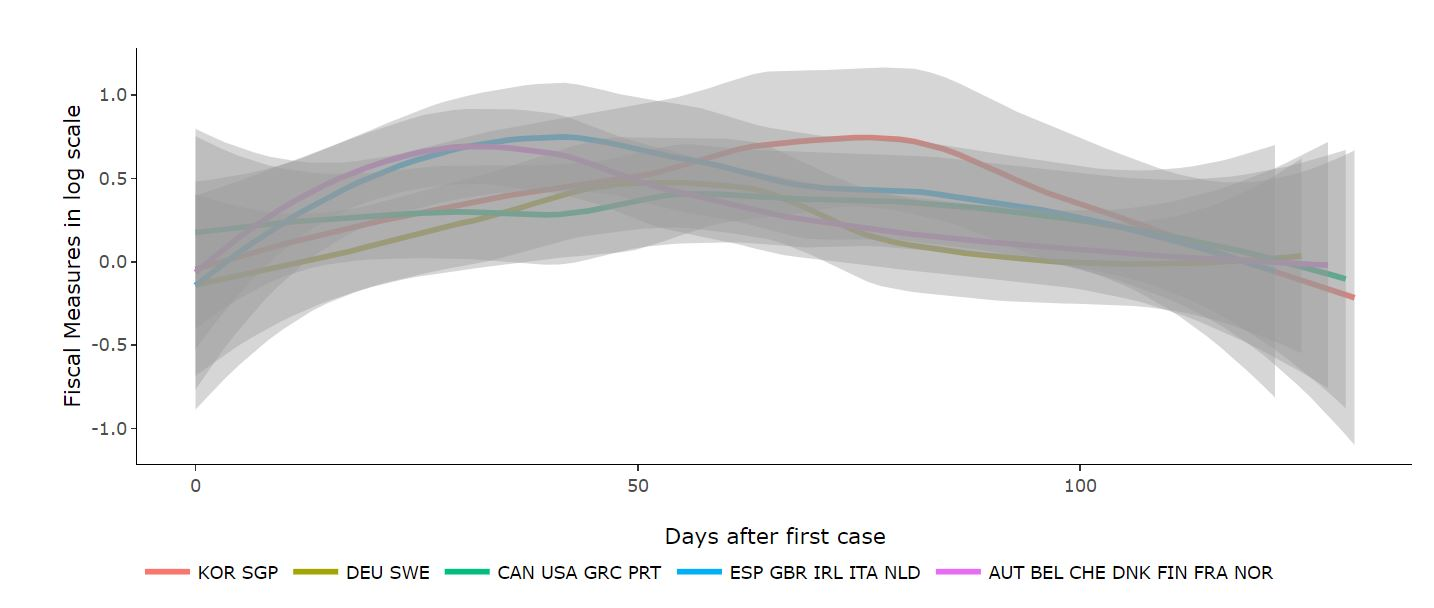
\includegraphics[width=\textwidth]{Report_SC_Group3_files/figure-latex/fig2.jpg}

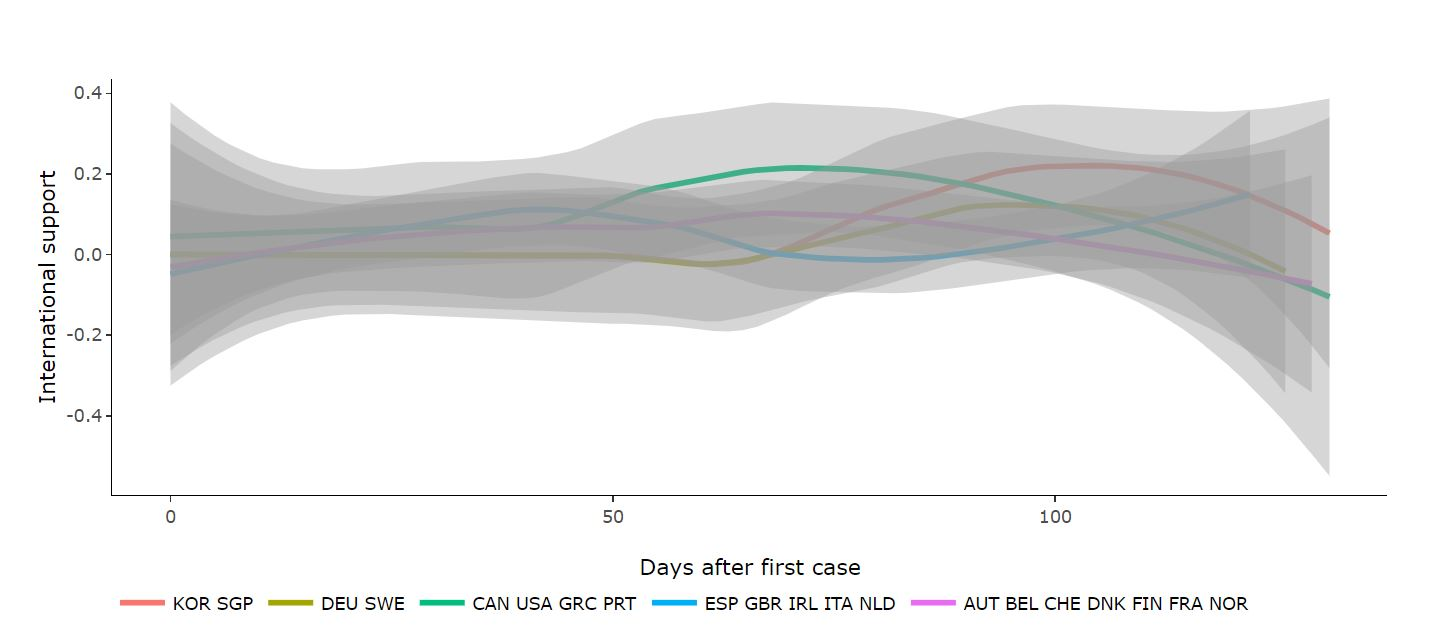
\includegraphics[width=\textwidth]{Report_SC_Group3_files/figure-latex/fig3.jpg}
\end{center}


The fiscal measure and international support variables have a large
within-clusters variability. As we will see, these two variables will
not enter into the final model.

For further details about the definition of the economic variables,
please see the
\href{https://www.bsg.ox.ac.uk/sites/default/files/2020-05/BSG-WP-2020-032-v5.0_0.pdf}{BSG
Working Paper Series}.

\hypertarget{demographiceconomichealth-system-fixed-variables}{%
\subsection{Demographic/economic/health system fixed
variables}\label{demographiceconomichealth-system-fixed-variables}}

We analyze \(8\) variables from the
\href{https://data.worldbank.org/}{World Bank Open Data} that are fixed
along the temporal dimension:

\begin{longtable}[]{@{}ll@{}}
\toprule
\textbf{Name} & \textbf{Measurement}\tabularnewline
\midrule
\endhead
Population & Numeric\tabularnewline
Population ages 65 and above (\% of total population) &
Numeric\tabularnewline
Population density (people per sq. km of land area) &
Numeric\tabularnewline
Hospital beds (per 1,000 people) & Numeric\tabularnewline
Death rate, crude (per 1,000 people) & Numeric\tabularnewline
GDP growth (annual \%) & Numeric\tabularnewline
Urban population (\% of total population) & Numeric\tabularnewline
Surface area (sq. km) & Numeric\tabularnewline
\bottomrule
\end{longtable}

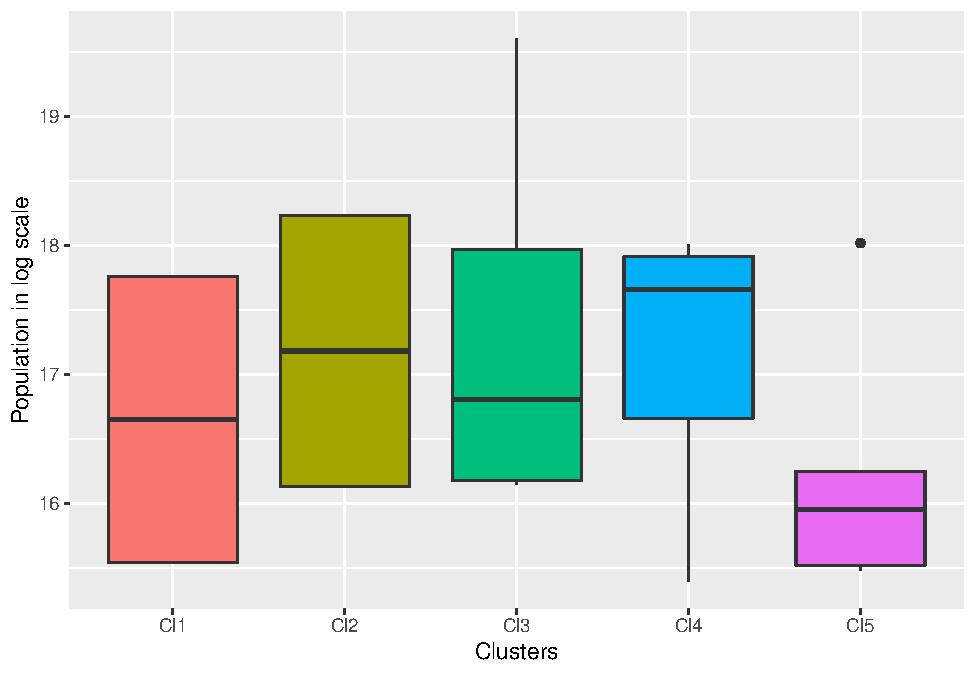
\includegraphics[width=.5\textwidth]{Report_SC_Group3_files/figure-latex/unnamed-chunk-8-1.pdf}
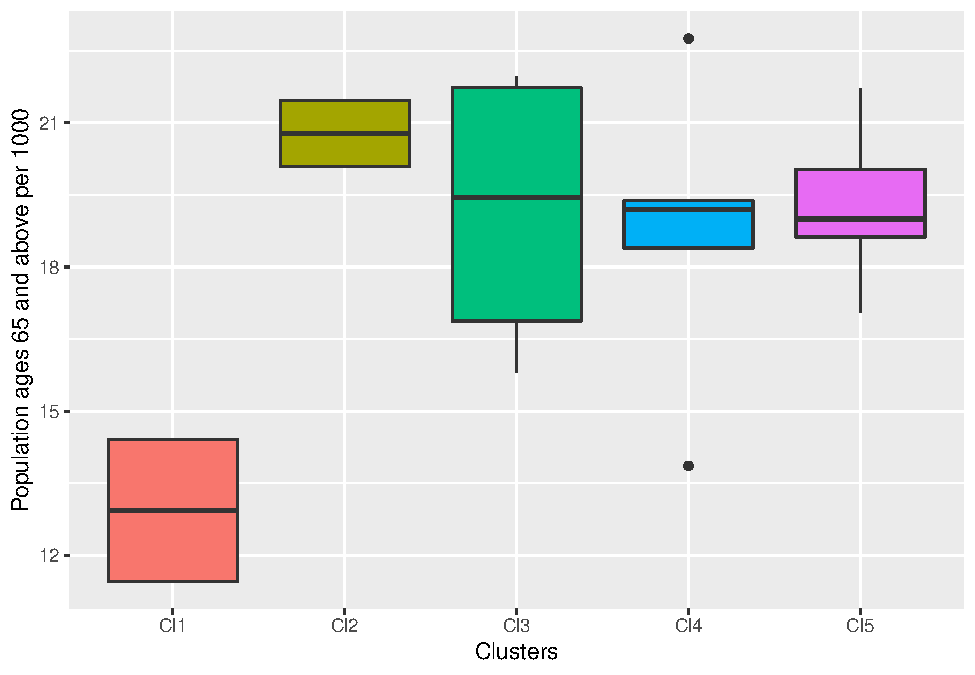
\includegraphics[width=.5\textwidth]{Report_SC_Group3_files/figure-latex/unnamed-chunk-8-2.pdf}

Korea and Singapore seem to be the two youngest countries; it could be a
reason for their low number of active people during the pandemic period.

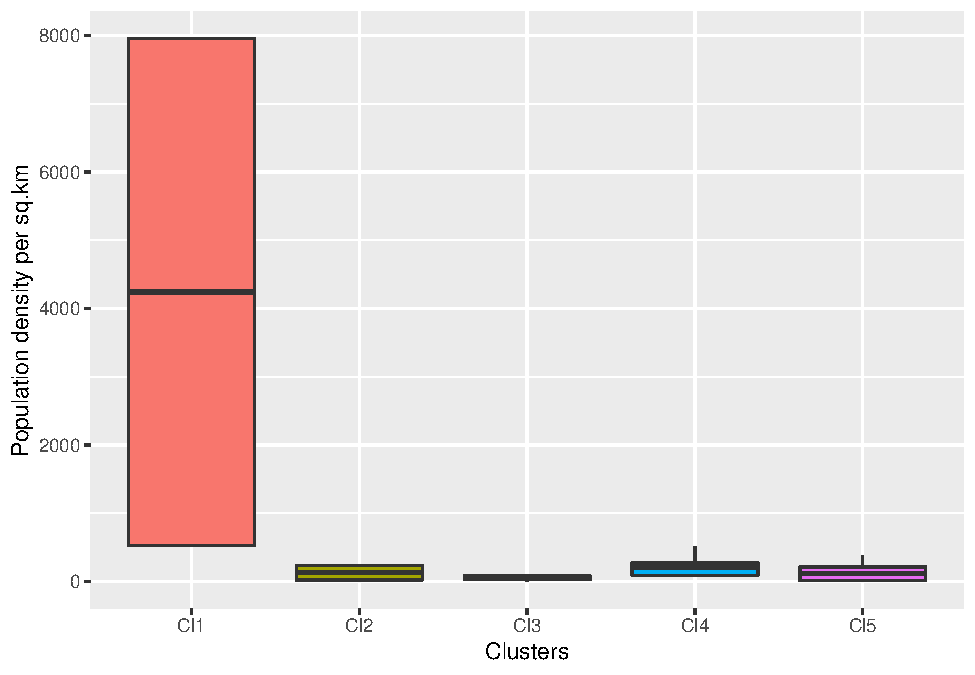
\includegraphics[width=.5\textwidth]{Report_SC_Group3_files/figure-latex/unnamed-chunk-9-1.pdf}
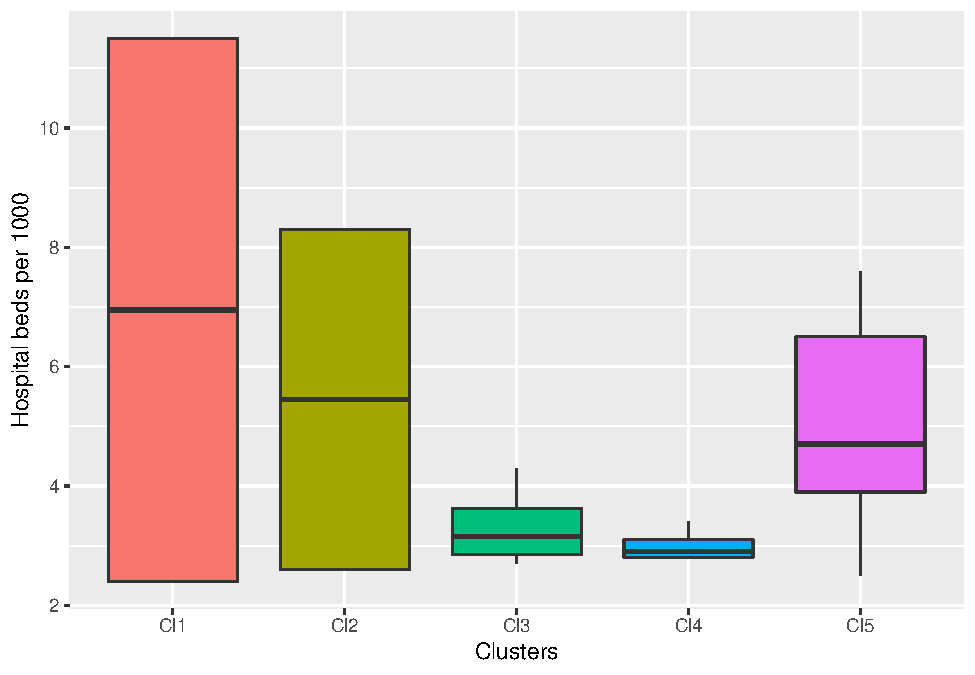
\includegraphics[width=.5\textwidth]{Report_SC_Group3_files/figure-latex/unnamed-chunk-9-2.pdf}

The population density of the first Cluster seems weird, it is due by
the Singapore situation. Probably, the number of hospital beds are
directly associated.

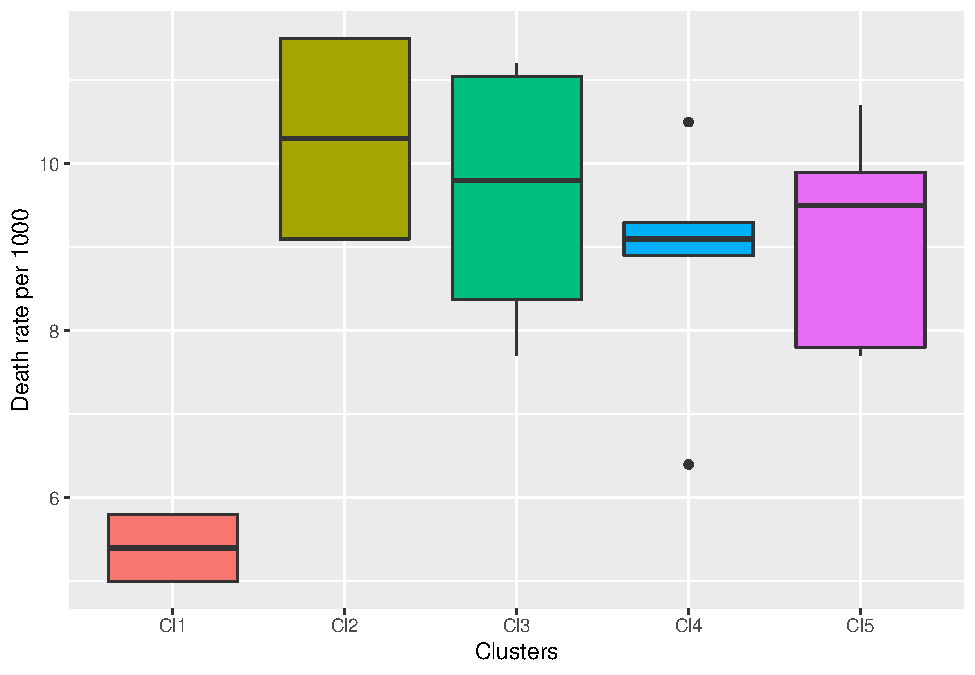
\includegraphics[width=.5\textwidth]{Report_SC_Group3_files/figure-latex/unnamed-chunk-10-1.pdf}
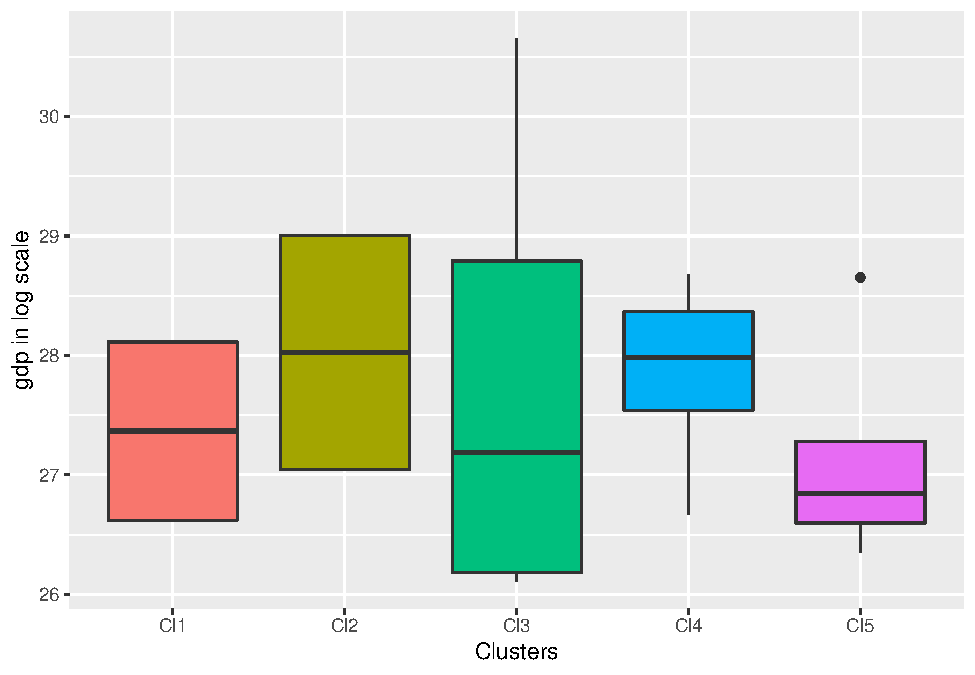
\includegraphics[width=.5\textwidth]{Report_SC_Group3_files/figure-latex/unnamed-chunk-10-2.pdf}

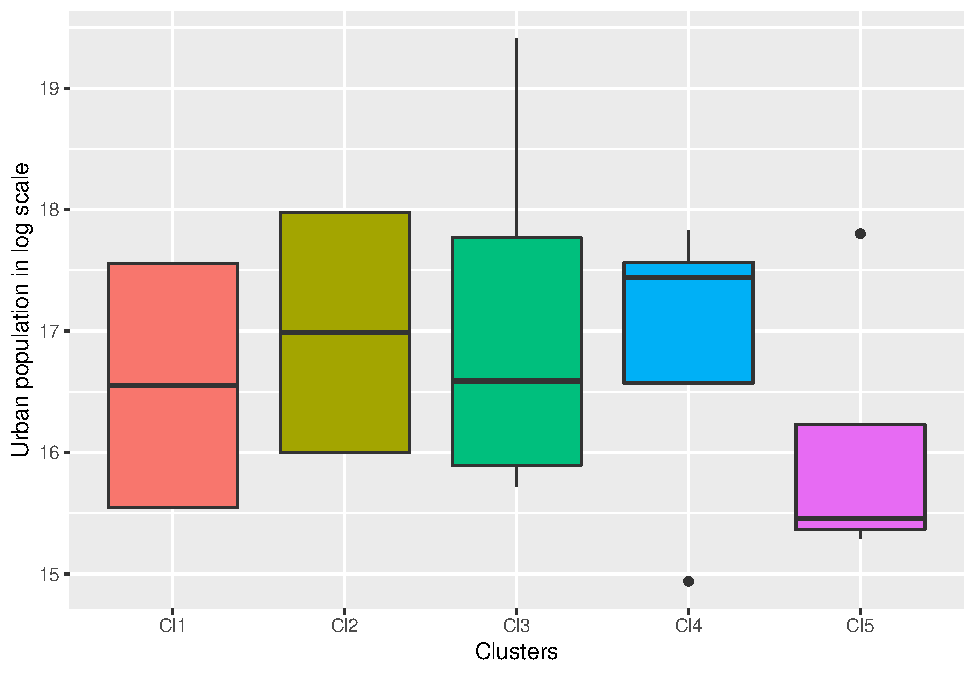
\includegraphics[width=.5\textwidth]{Report_SC_Group3_files/figure-latex/unnamed-chunk-11-1.pdf}
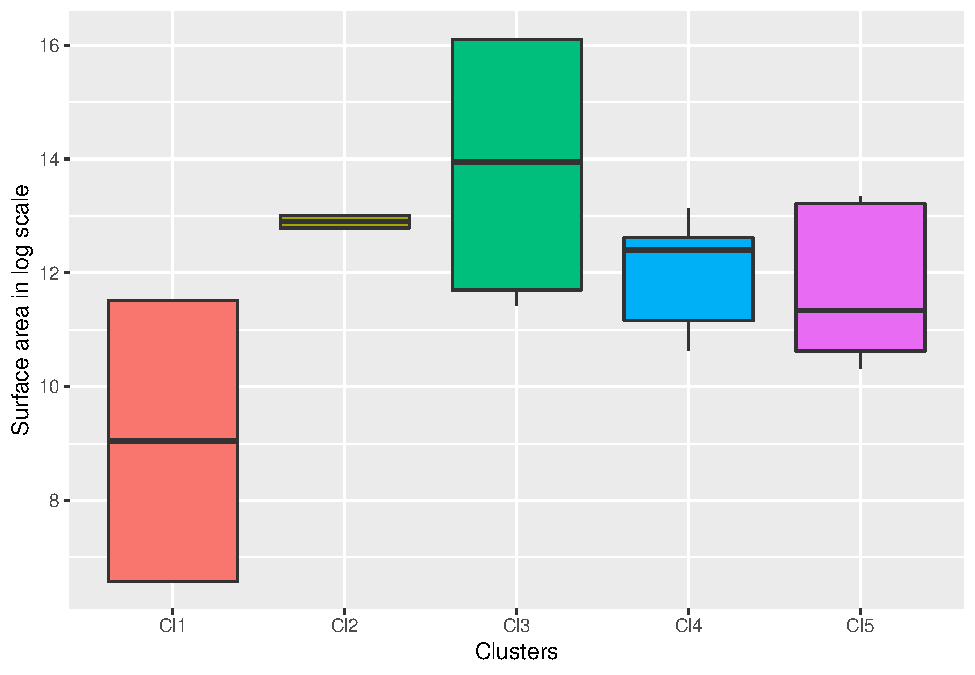
\includegraphics[width=.5\textwidth]{Report_SC_Group3_files/figure-latex/unnamed-chunk-11-2.pdf}

Another time the Singapore situation is clear analyzing the first
Cluster. We have a large density population, so lower surface area than
the ones of the other countries.

\hypertarget{longitudinal-health-system-variables}{%
\subsection{Longitudinal health system
variables}\label{longitudinal-health-system-variables}}

We analyze \(2\) health systems' variables from Thomas et al. (2020):

\begin{longtable}[]{@{}lll@{}}
\toprule
\begin{minipage}[b]{0.30\columnwidth}\raggedright
\textbf{Name}\strut
\end{minipage} & \begin{minipage}[b]{0.2\columnwidth}\raggedright
\textbf{Measurement} \strut
\end{minipage} & \begin{minipage}[b]{0.4\columnwidth}\raggedright
\textbf{Description}\strut
\end{minipage}\tabularnewline
\midrule
\endhead
\begin{minipage}[t]{0.4\columnwidth}\raggedright
Emergency Investment in healthcare\strut
\end{minipage} & \begin{minipage}[t]{0.11\columnwidth}\raggedright
USD\strut
\end{minipage} & \begin{minipage}[t]{0.47\columnwidth}\raggedright
Short-term spending on, e.g, hospitals, masks, etc\strut
\end{minipage}\tabularnewline
\begin{minipage}[t]{0.33\columnwidth}\raggedright
Investment in vaccines\strut
\end{minipage} & \begin{minipage}[t]{0.11\columnwidth}\raggedright
USD\strut
\end{minipage} & \begin{minipage}[t]{0.47\columnwidth}\raggedright
Announced public spending on vaccine development\strut
\end{minipage}\tabularnewline
\bottomrule
\end{longtable}

The set of the health systems' variables are transformed into one
continuous variable using the Polychoric Principal Component Analysis,
in order to reduce the number of covariates in the model.
\begin{center}
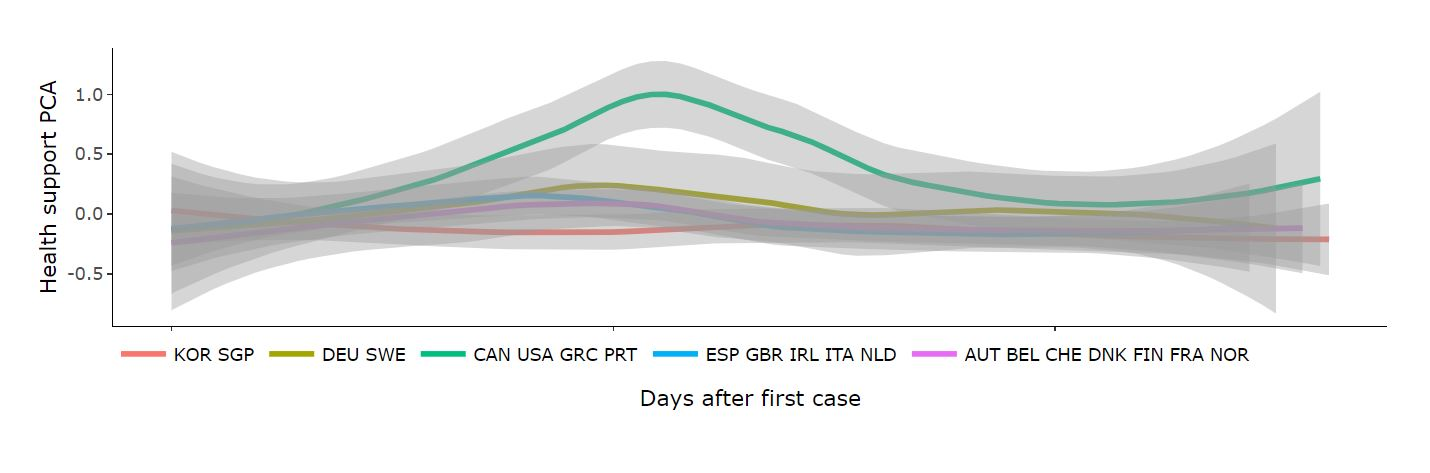
\includegraphics[width=\textwidth]{Report_SC_Group3_files/figure-latex/fig4.jpg}
\end{center}
\hypertarget{containment-strategies-and-resembling-patterns}{%
\section{Containment strategies and resembling
patterns}\label{containment-strategies-and-resembling-patterns}}

Identification and codification of different measures undertaken by
governments performed by the University of Oxford result in \(11\)
ordinal variables selected as lockdown policies. This situation sets up
the necessity to analyze and aggregate them in a synthetic way to find
out whether specific combinations of those policies making up political
strategies come out to have a resemblance pattern across countries.

Therefore, we performed a Principal Component Analysis based on the
polychoric correlation. It allows the estimation of the correlation
between two theorized normally distributed continuous latent variables,
from two observed ordinal variables. It has no closed-form, but it is
estimated via MLE assuming the two latent variables follow a bivariate
normal density.

The interpretation of the first three principal components (accounting
for the 80\% of total variance) appears to be clear in the following
figure: the first one is closely related with freedom of movements and
gathering restrictions together with information campaigns strategy,
crucial in cases of draconian measures, the second one is related with
the strategy of informing and testing the population, lastly the third
one is related to informing and contact tracing the population.
Summarizing, on one hand a first containment strategy aims at social
distancing the entire population, on the other hand a second one aims at
act locally and rapidly detect and isolate the positive cases, with two
(alternative or complementary) tools: tracing contacts of infected
and/or blanket population testing.

\begin{figure}
\centering
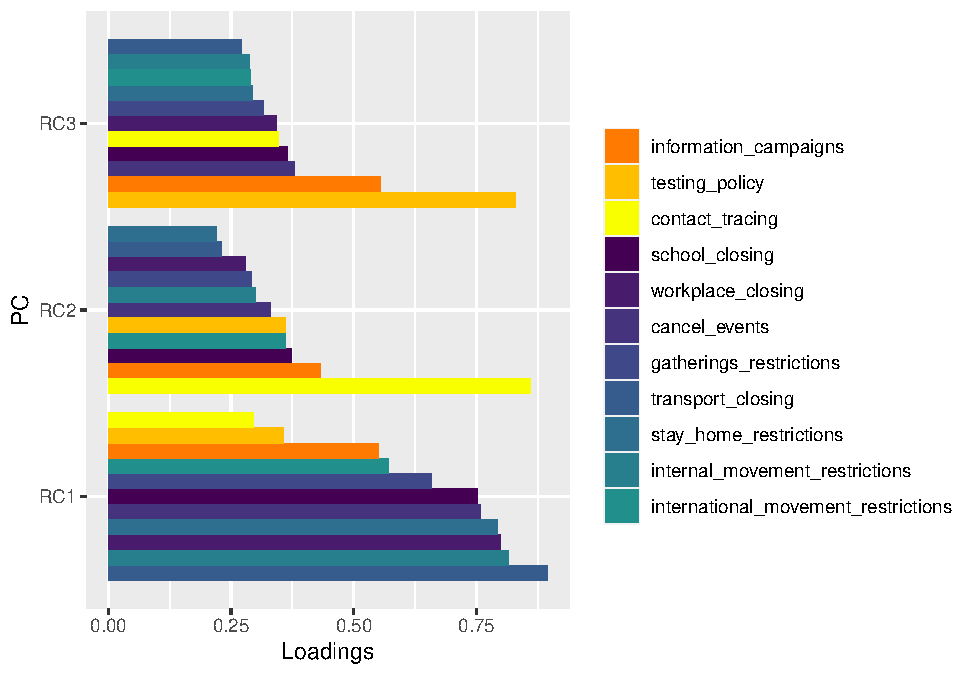
\includegraphics{Report_SC_Group3_files/figure-latex/figs-1.pdf}
\caption{\label{fig:figs}First 3 Principal Components Loadings.}
\end{figure}

We want now to figure out which countries have adopted the undefined
strategies and whether there is a strategy resemblance across countries,
considering both the combination of measures undertaken and the timing
w.r.t. the day of the first contagion detection on country soil. In
order to do so, we performed a functional co-clustering of the first
three principal components taking into account 20 countries in a
specific time span (which varies from country to country) that depends
on when the first COVID cases have been detected on national soil. We
performed an alignment of the contagion pattern from the 10th day before
first contagion detection to include relevant information on the
prevention measures.

Considering a matrix of 20 countries (rows) of 3 curves (columns or
functional features- restriction-based, testing-based, and tracing-based
policies) s.t. \(x=(x_{ij}(t))_{1\leq i \leq 20; 1 \leq j\leq3}\) with
\(t \in [0,85]\), we reconstructed the functional form of the data from
their discrete observations (85 days) by assuming that curves belong to
a finite-dimensional space spanned by a basis of functions, and then we
estimated a functional latent block model used for co-clustering with
the funFEM R package developed by Bouveyron and Jacques (2015).

The two policy clusters depict Restriction-based policies on one hand,
Tracing, and Testing-based policies, on the other hand, confirming that
these last two policies reflect a common strategy as described above.

The countries clusters are displayed in the following figures: (South
Korea, Singapore), (Germany, Sweden), (USA, Canada, Greece, Portugal),
(Italy, Spain, Ireland, UK, Netherlands), (Norway, Denmark, Finland,
France, Belgium, Switzerland, Austria). The interpretation can be
grasped in the following figure. South Korea and Singapore's political
strategy is characterized by the detection and isolation of the positive
cases via contact tracing and mild testing policies, without any
relevant social distancing action. On the contrary, Germany, Sweden's
strategy was to detect and isolate positive cases via an extensive
testing policy strategy, without any strong social distancing measures
in order to protect the economy. A very different strategy has been
adopted by the cluster, including Italy, Spain, Ireland, UK, and
Netherlands, which acted with social distancing measures at different
temporal stages (considering, in particular, the north European
countries of the cluster) but promptly concerning the first contagion
inside national borders. In particular, the strategies of Ireland, UK,
and the Netherland were stringent concerning school and workplace
closing as well as gathering and international movement restriction,
weaker as regards stay at home recommendations, internal movement
restriction, and transport closing but at the same time relying on a
strong information campaign. On the other hand, Italy and Spain
sharpened up stay at home and internal movement restrictions. USA,
Canada, Greece, and Portugal have adopted intermittently social
distancing measures in addition with strong social tracing during the
second part of the considered period. Lastly, Norway, Denmark, Finland,
France, Belgium, Switzerland, Austria has adopted intermediate social
distancing measure, in line with other European countries, but without
any relevant testing or tracing measure in addition.

\begin{figure}
\centering
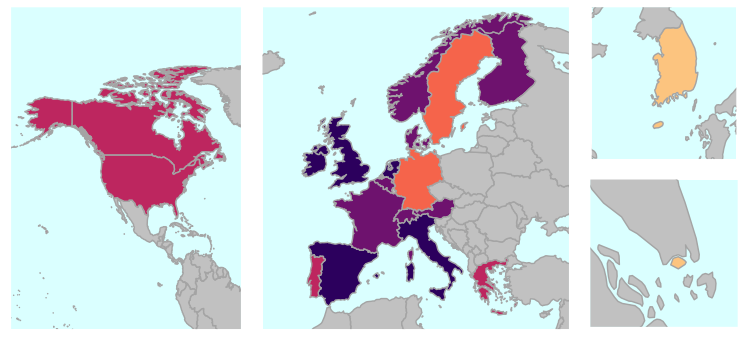
\includegraphics{maps.png}
\caption{Clusters map.}
\end{figure}

\begin{figure}

{\centering 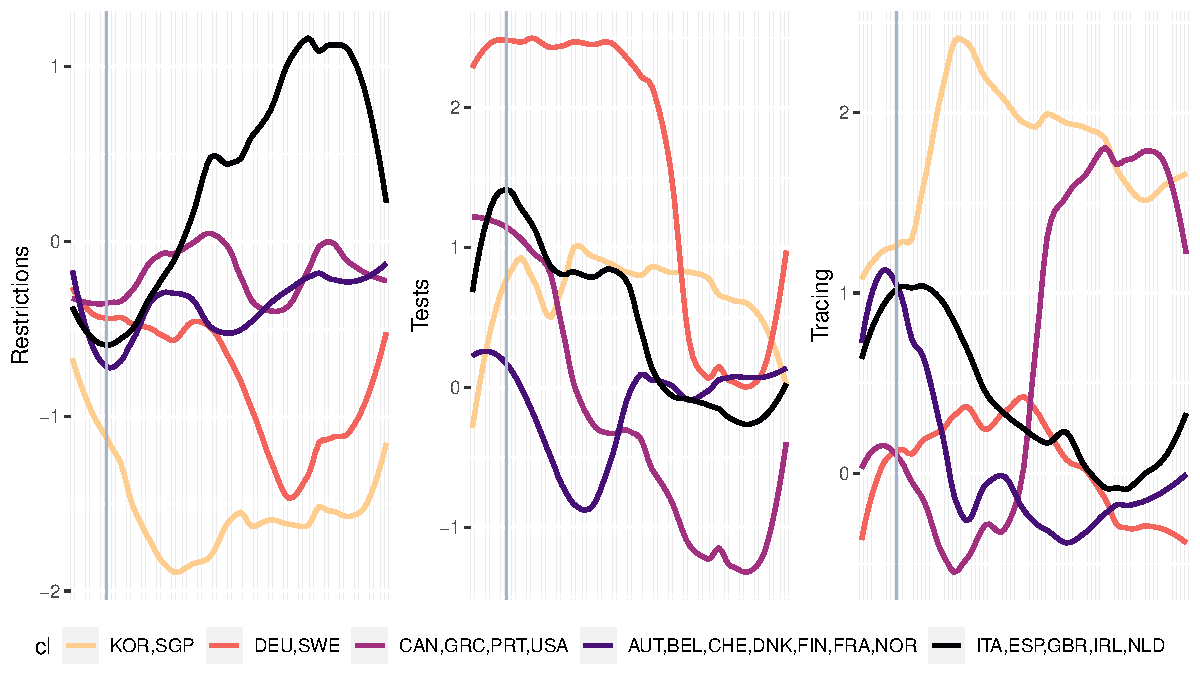
\includegraphics{Report_SC_Group3_files/figure-latex/figs3-1} 

}

\caption{\label{fig:figs3}Clusters average functionals related to Social Distancing Restrinction, Testing and Tracing policies aligned at the day of the first contagion (vertical blue line).}\label{fig:figs3}
\end{figure}

\hypertarget{effect-of-policies-from-a-global-perspective}{%
\section{Effect of policies from a global
perspective}\label{effect-of-policies-from-a-global-perspective}}

We want to analyze which countries have adopted the ``optimal'' policy
measures to contain the contagion of COVID-19. We restrict the full
range of responses to COVID-19 from governments around the countries
analyzed in Section 3, i.e., Korea, Singapore, Germany, Canada, Sweden,
Greece, Portugal, Spain, United States of America, Irland, United
Kingdom, Italy, Netherlands, Austria, Switzerland, Finland, Norway,
Denmark, and France.

The daily number of active persons is analyzed as a measure of the
COVID-19 situation, i.e., the number of confirmed minus the number of
deaths minus the number of recovered. Being a count variable, we decide
to use a Negative Binomial Regression, also correcting for the possible
overdispersion. Therefore, the hierarchical structure is induced by the
structure of countries nested inside the clusters and by the
longitudinal structure. For that, we decide to use a generalized mixed
model with family negative binomial. The countries, clusters, and date's
information are supposed to be used as random effects in the model. The
indicators from Thomas et al. (2020) and the demographic/economic/health
variables from the \href{https://data.worldbank.org/}{World Bank Open
Data} enter as fixed effects in the model.

So, the aim is to understand how the lockdown policies influence the
number of active people. The observations are aligned concerning the
first active case across the countries to have observations directly
comparable from a longitudinal point of view. The following Figure
represents the number of active people during \(131\) days for each
country, and the corresponding mean value of the clusters.

\begin{figure}
\centering
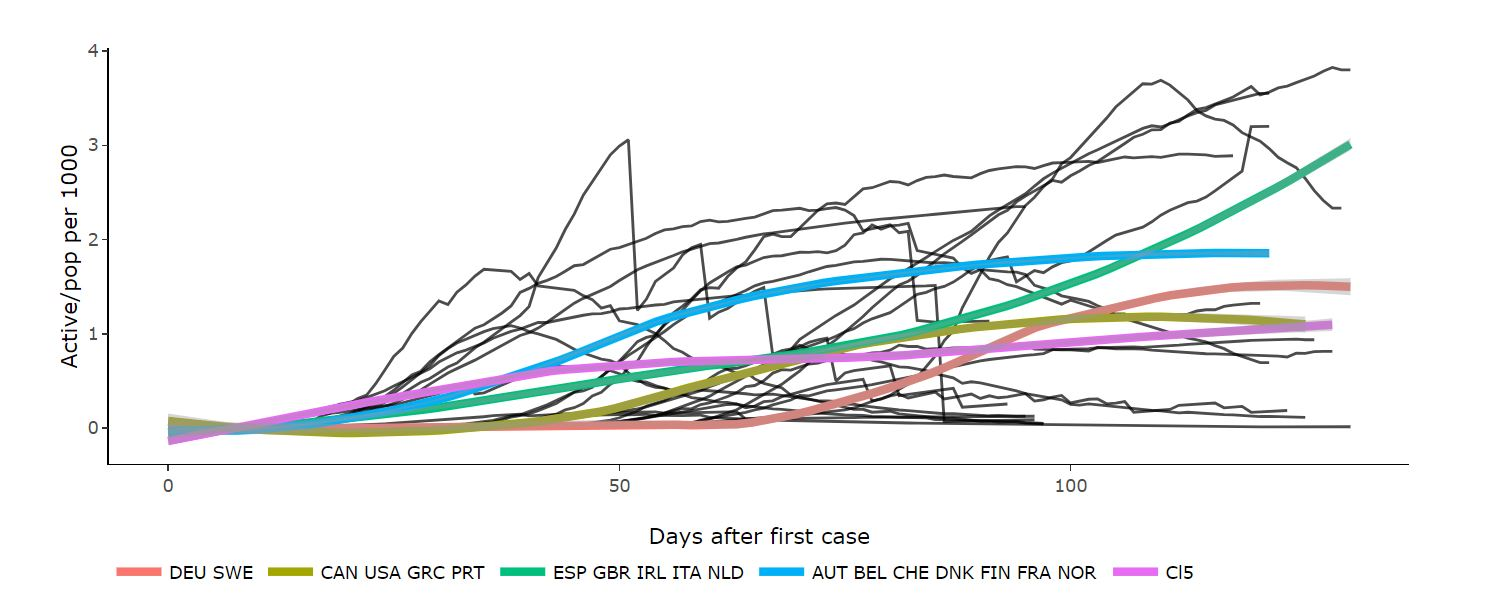
\includegraphics[width=\textwidth]{Report_SC_Group3_files/figure-latex/fig5.jpg}
\caption{\label{fig:figsA1} Number of active people over population
across time for each countries. The mean of each cluster is also
displayed.}
\end{figure}

The temporal variability between countries and clusters is clear, as
confirmation about the decision to use the generalized mixed model.

\hypertarget{model}{%
\subsection{Model}\label{model}}

The aim is to model the number of active people, i.e., confirmed -
deaths - recovered, after \(14\) days, when the lockdown policies were
applied. Therefore, the number of \textbf{active people lagged} to
\(t+14\) days, and an \textbf{offset term} representing the number of
active people at time \(t\) are considered to analyze the influences of
the restrictions imposed at time \(t\) on the number of active at time
\(t+14\).

The data has a \textbf{three-level structure}. The variability of the
data comes from nested sources: countries are nested within clusters,
and the observations are repeated across time, i.e., longitudinal data.

For that, the mixed model approach is considered to exploit the
different types of variability coming from the hierarchical data
structure. At first, the Intraclass Correlation Coefficient (ICC) is
computed:

\[
ICC_{date; active} = 0.0936 \quad ICC_{Countries; Active} = 0.4015 \quad ICC_{Clusters; Active} = 0.0951 
\]

Therefore, the \(40.15\%\) of the data's variance is given by the random
effect of the countries, while the \(9.36\%\) by the temporal effect and
\(9.51\%\) by the clusters effect. Therefore, the mixed model requires a
random effect for the countries; the other two effects are selected
using the conditional AIC.

The dependent variable is the number of active persons; therefore, a
count data model is considered. To control the overdispersion of our
data, the negative binomial regression with Gaussian-distributed random
effects is performed using the glmmTMB R package developed by Brooks et
al. (2017). Let \(n\) countries, and country \(i\) is measured at
\(n_i\) time points. The active person \(y_{ij}\) count at time
\(t+14\), where \(i=1,\dots, n\) and \(j = 1, \dots,n_i\), follows the
negative binomial distribution:

\[y_{ij} \sim NB(y_{ij}|\mu_{ij}, \theta) = \dfrac{\Gamma(y_{ij}+ \theta)}{\Gamma(\theta) y_{ij}!} \cdot \Big(\dfrac{\theta}{\mu_{ij} + \theta}\Big)^{\theta}\cdot \Big(\dfrac{\mu_{ij}}{\mu_{ij} + \theta}\Big)^{y_{ij}}\]
where \(\theta\) is the dispersion parameter that controls the amount of
overdispersion, and \(\mu_{ij}\) are the means. The means \(\mu_{ij}\)
are related to the other variables via the logarithm link function:

\[\log(\mu_{ij}) = \log(T_{ij}) + X_{ij} \beta + Z_{ij} b_i \quad b_i \sim \mathcal{N}(0,\psi)\]

where \(\log(T_{ij})\) is the offset that corrects for the variation of
the count of the active person at time \(t\), and
\(\text{E}(y_{ij}) = \mu_{ij}\),
\(\text{Var}(y_{ij}) = \mu_{ij} (1 + \mu_{ij}\theta)\) from Hardin and
Hilbe (2018). The \(X_{ij}\) is the design matrix for the fixed effects,
i.e., economic, demographic and health variables (the confounders
described in section 2), and \(\beta\) the corresponding set of fixed
parameters. In the same way, \(Z_{ij}\) is the design matrix describing
the random effect regarding the countries and the date, and \(b_i\) the
corresponding parameter.

After some covariates selection steps and random effects selection, the
final model returns these estimations for the fixed effects:

\begin{longtable}[]{@{}lrrrr@{}}
\toprule
\begin{minipage}[b]{0.47\columnwidth}\raggedright
\strut
\end{minipage} & \begin{minipage}[b]{0.07\columnwidth}\raggedleft
Estimate\strut
\end{minipage} & \begin{minipage}[b]{0.09\columnwidth}\raggedleft
Std. Error\strut
\end{minipage} & \begin{minipage}[b]{0.07\columnwidth}\raggedleft
z value\strut
\end{minipage} & \begin{minipage}[b]{0.16\columnwidth}\raggedleft
Pr(\textgreater\textbar z\textbar)\strut
\end{minipage}\tabularnewline
\midrule
\endhead
\begin{minipage}[t]{0.47\columnwidth}\raggedright
Intercept\strut
\end{minipage} & \begin{minipage}[t]{0.07\columnwidth}\raggedleft
-0.012\strut
\end{minipage} & \begin{minipage}[t]{0.09\columnwidth}\raggedleft
0.326\strut
\end{minipage} & \begin{minipage}[t]{0.07\columnwidth}\raggedleft
-0.035\strut
\end{minipage} & \begin{minipage}[t]{0.16\columnwidth}\raggedleft
0.972\strut
\end{minipage}\tabularnewline
\begin{minipage}[t]{0.47\columnwidth}\raggedright
Economic PCA\strut
\end{minipage} & \begin{minipage}[t]{0.07\columnwidth}\raggedleft
-0.547\strut
\end{minipage} & \begin{minipage}[t]{0.09\columnwidth}\raggedleft
0.070\strut
\end{minipage} & \begin{minipage}[t]{0.07\columnwidth}\raggedleft
-7.791\strut
\end{minipage} & \begin{minipage}[t]{0.16\columnwidth}\raggedleft
0.000\strut
\end{minipage}\tabularnewline
\begin{minipage}[t]{0.47\columnwidth}\raggedright
Population density in log scale\strut
\end{minipage} & \begin{minipage}[t]{0.07\columnwidth}\raggedleft
0.103\strut
\end{minipage} & \begin{minipage}[t]{0.09\columnwidth}\raggedleft
0.031\strut
\end{minipage} & \begin{minipage}[t]{0.07\columnwidth}\raggedleft
3.354\strut
\end{minipage} & \begin{minipage}[t]{0.16\columnwidth}\raggedleft
0.001\strut
\end{minipage}\tabularnewline
\begin{minipage}[t]{0.47\columnwidth}\raggedright
Health System PCA\strut
\end{minipage} & \begin{minipage}[t]{0.07\columnwidth}\raggedleft
0.053\strut
\end{minipage} & \begin{minipage}[t]{0.09\columnwidth}\raggedleft
0.020\strut
\end{minipage} & \begin{minipage}[t]{0.07\columnwidth}\raggedleft
2.607\strut
\end{minipage} & \begin{minipage}[t]{0.16\columnwidth}\raggedleft
0.009\strut
\end{minipage}\tabularnewline
\begin{minipage}[t]{0.47\columnwidth}\raggedright
Recommend closing workplace\strut
\end{minipage} & \begin{minipage}[t]{0.07\columnwidth}\raggedleft
-0.290\strut
\end{minipage} & \begin{minipage}[t]{0.09\columnwidth}\raggedleft
0.138\strut
\end{minipage} & \begin{minipage}[t]{0.07\columnwidth}\raggedleft
-2.108\strut
\end{minipage} & \begin{minipage}[t]{0.16\columnwidth}\raggedleft
0.035\strut
\end{minipage}\tabularnewline
\begin{minipage}[t]{0.47\columnwidth}\raggedright
Require closing workplace\strut
\end{minipage} & \begin{minipage}[t]{0.07\columnwidth}\raggedleft
-1.191\strut
\end{minipage} & \begin{minipage}[t]{0.09\columnwidth}\raggedleft
0.134\strut
\end{minipage} & \begin{minipage}[t]{0.07\columnwidth}\raggedleft
-8.902\strut
\end{minipage} & \begin{minipage}[t]{0.16\columnwidth}\raggedleft
0.000\strut
\end{minipage}\tabularnewline
\begin{minipage}[t]{0.47\columnwidth}\raggedright
Require closing workplace all-but-essential workplaces\strut
\end{minipage} & \begin{minipage}[t]{0.07\columnwidth}\raggedleft
-0.513\strut
\end{minipage} & \begin{minipage}[t]{0.09\columnwidth}\raggedleft
0.170\strut
\end{minipage} & \begin{minipage}[t]{0.07\columnwidth}\raggedleft
-3.021\strut
\end{minipage} & \begin{minipage}[t]{0.16\columnwidth}\raggedleft
0.003\strut
\end{minipage}\tabularnewline
\begin{minipage}[t]{0.47\columnwidth}\raggedright
Restrictions on gatherings \textless1000 people\strut
\end{minipage} & \begin{minipage}[t]{0.07\columnwidth}\raggedleft
-0.506\strut
\end{minipage} & \begin{minipage}[t]{0.09\columnwidth}\raggedleft
0.162\strut
\end{minipage} & \begin{minipage}[t]{0.07\columnwidth}\raggedleft
-3.120\strut
\end{minipage} & \begin{minipage}[t]{0.16\columnwidth}\raggedleft
0.002\strut
\end{minipage}\tabularnewline
\begin{minipage}[t]{0.47\columnwidth}\raggedright
Restrictions on gatherings between 101-1000 people\strut
\end{minipage} & \begin{minipage}[t]{0.07\columnwidth}\raggedleft
-1.259\strut
\end{minipage} & \begin{minipage}[t]{0.09\columnwidth}\raggedleft
0.141\strut
\end{minipage} & \begin{minipage}[t]{0.07\columnwidth}\raggedleft
-8.945\strut
\end{minipage} & \begin{minipage}[t]{0.16\columnwidth}\raggedleft
0.000\strut
\end{minipage}\tabularnewline
\begin{minipage}[t]{0.47\columnwidth}\raggedright
Restrictions on gatherings between 11-100 people\strut
\end{minipage} & \begin{minipage}[t]{0.07\columnwidth}\raggedleft
-1.519\strut
\end{minipage} & \begin{minipage}[t]{0.09\columnwidth}\raggedleft
0.173\strut
\end{minipage} & \begin{minipage}[t]{0.07\columnwidth}\raggedleft
-8.804\strut
\end{minipage} & \begin{minipage}[t]{0.16\columnwidth}\raggedleft
0.000\strut
\end{minipage}\tabularnewline
\begin{minipage}[t]{0.47\columnwidth}\raggedright
Restrictions on gatherings of \textless{} 10 people\strut
\end{minipage} & \begin{minipage}[t]{0.07\columnwidth}\raggedleft
-1.702\strut
\end{minipage} & \begin{minipage}[t]{0.09\columnwidth}\raggedleft
0.179\strut
\end{minipage} & \begin{minipage}[t]{0.07\columnwidth}\raggedleft
-9.513\strut
\end{minipage} & \begin{minipage}[t]{0.16\columnwidth}\raggedleft
0.000\strut
\end{minipage}\tabularnewline
\begin{minipage}[t]{0.47\columnwidth}\raggedright
Recommend transport closing\strut
\end{minipage} & \begin{minipage}[t]{0.07\columnwidth}\raggedleft
-0.056\strut
\end{minipage} & \begin{minipage}[t]{0.09\columnwidth}\raggedleft
0.106\strut
\end{minipage} & \begin{minipage}[t]{0.07\columnwidth}\raggedleft
-0.527\strut
\end{minipage} & \begin{minipage}[t]{0.16\columnwidth}\raggedleft
0.598\strut
\end{minipage}\tabularnewline
\begin{minipage}[t]{0.47\columnwidth}\raggedright
Require transport closing\strut
\end{minipage} & \begin{minipage}[t]{0.07\columnwidth}\raggedleft
-0.501\strut
\end{minipage} & \begin{minipage}[t]{0.09\columnwidth}\raggedleft
0.198\strut
\end{minipage} & \begin{minipage}[t]{0.07\columnwidth}\raggedleft
-2.529\strut
\end{minipage} & \begin{minipage}[t]{0.16\columnwidth}\raggedleft
0.011\strut
\end{minipage}\tabularnewline
\begin{minipage}[t]{0.47\columnwidth}\raggedright
Recommend not leaving house\strut
\end{minipage} & \begin{minipage}[t]{0.07\columnwidth}\raggedleft
-0.057\strut
\end{minipage} & \begin{minipage}[t]{0.09\columnwidth}\raggedleft
0.109\strut
\end{minipage} & \begin{minipage}[t]{0.07\columnwidth}\raggedleft
-0.528\strut
\end{minipage} & \begin{minipage}[t]{0.16\columnwidth}\raggedleft
0.598\strut
\end{minipage}\tabularnewline
\begin{minipage}[t]{0.47\columnwidth}\raggedright
Require not leaving house (only essential trips)\strut
\end{minipage} & \begin{minipage}[t]{0.07\columnwidth}\raggedleft
-0.111\strut
\end{minipage} & \begin{minipage}[t]{0.09\columnwidth}\raggedleft
0.148\strut
\end{minipage} & \begin{minipage}[t]{0.07\columnwidth}\raggedleft
-0.751\strut
\end{minipage} & \begin{minipage}[t]{0.16\columnwidth}\raggedleft
0.453\strut
\end{minipage}\tabularnewline
\begin{minipage}[t]{0.47\columnwidth}\raggedright
Require not leaving house with minimal exceptions\strut
\end{minipage} & \begin{minipage}[t]{0.07\columnwidth}\raggedleft
-0.824\strut
\end{minipage} & \begin{minipage}[t]{0.09\columnwidth}\raggedleft
0.292\strut
\end{minipage} & \begin{minipage}[t]{0.07\columnwidth}\raggedleft
-2.826\strut
\end{minipage} & \begin{minipage}[t]{0.16\columnwidth}\raggedleft
0.005\strut
\end{minipage}\tabularnewline
\begin{minipage}[t]{0.47\columnwidth}\raggedright
Testing only who both have symptoms and specific criteria\strut
\end{minipage} & \begin{minipage}[t]{0.07\columnwidth}\raggedleft
0.216\strut
\end{minipage} & \begin{minipage}[t]{0.09\columnwidth}\raggedleft
0.091\strut
\end{minipage} & \begin{minipage}[t]{0.07\columnwidth}\raggedleft
2.376\strut
\end{minipage} & \begin{minipage}[t]{0.16\columnwidth}\raggedleft
0.017\strut
\end{minipage}\tabularnewline
\begin{minipage}[t]{0.47\columnwidth}\raggedright
Testing everyone with symptoms\strut
\end{minipage} & \begin{minipage}[t]{0.07\columnwidth}\raggedleft
0.558\strut
\end{minipage} & \begin{minipage}[t]{0.09\columnwidth}\raggedleft
0.113\strut
\end{minipage} & \begin{minipage}[t]{0.07\columnwidth}\raggedleft
4.945\strut
\end{minipage} & \begin{minipage}[t]{0.16\columnwidth}\raggedleft
0.000\strut
\end{minipage}\tabularnewline
\begin{minipage}[t]{0.47\columnwidth}\raggedright
Open public testing\strut
\end{minipage} & \begin{minipage}[t]{0.07\columnwidth}\raggedleft
1.349\strut
\end{minipage} & \begin{minipage}[t]{0.09\columnwidth}\raggedleft
0.158\strut
\end{minipage} & \begin{minipage}[t]{0.07\columnwidth}\raggedleft
8.544\strut
\end{minipage} & \begin{minipage}[t]{0.16\columnwidth}\raggedleft
0.000\strut
\end{minipage}\tabularnewline
\begin{minipage}[t]{0.47\columnwidth}\raggedright
Limited tracing\strut
\end{minipage} & \begin{minipage}[t]{0.07\columnwidth}\raggedleft
0.196\strut
\end{minipage} & \begin{minipage}[t]{0.09\columnwidth}\raggedleft
0.083\strut
\end{minipage} & \begin{minipage}[t]{0.07\columnwidth}\raggedleft
2.369\strut
\end{minipage} & \begin{minipage}[t]{0.16\columnwidth}\raggedleft
0.018\strut
\end{minipage}\tabularnewline
\begin{minipage}[t]{0.47\columnwidth}\raggedright
Comprehensive tracing\strut
\end{minipage} & \begin{minipage}[t]{0.07\columnwidth}\raggedleft
0.360\strut
\end{minipage} & \begin{minipage}[t]{0.09\columnwidth}\raggedleft
0.095\strut
\end{minipage} & \begin{minipage}[t]{0.07\columnwidth}\raggedleft
3.784\strut
\end{minipage} & \begin{minipage}[t]{0.16\columnwidth}\raggedleft
0.000\strut
\end{minipage}\tabularnewline
\begin{minipage}[t]{0.47\columnwidth}\raggedright
DEU SWE\strut
\end{minipage} & \begin{minipage}[t]{0.07\columnwidth}\raggedleft
1.461\strut
\end{minipage} & \begin{minipage}[t]{0.09\columnwidth}\raggedleft
0.173\strut
\end{minipage} & \begin{minipage}[t]{0.07\columnwidth}\raggedleft
8.454\strut
\end{minipage} & \begin{minipage}[t]{0.16\columnwidth}\raggedleft
0.000\strut
\end{minipage}\tabularnewline
\begin{minipage}[t]{0.47\columnwidth}\raggedright
CAN USA GRC PRT\strut
\end{minipage} & \begin{minipage}[t]{0.07\columnwidth}\raggedleft
1.955\strut
\end{minipage} & \begin{minipage}[t]{0.09\columnwidth}\raggedleft
0.158\strut
\end{minipage} & \begin{minipage}[t]{0.07\columnwidth}\raggedleft
12.377\strut
\end{minipage} & \begin{minipage}[t]{0.16\columnwidth}\raggedleft
0.000\strut
\end{minipage}\tabularnewline
\begin{minipage}[t]{0.47\columnwidth}\raggedright
ESP GBR IRL ITA NLD\strut
\end{minipage} & \begin{minipage}[t]{0.07\columnwidth}\raggedleft
2.365\strut
\end{minipage} & \begin{minipage}[t]{0.09\columnwidth}\raggedleft
0.148\strut
\end{minipage} & \begin{minipage}[t]{0.07\columnwidth}\raggedleft
16.029\strut
\end{minipage} & \begin{minipage}[t]{0.16\columnwidth}\raggedleft
0.000\strut
\end{minipage}\tabularnewline
\begin{minipage}[t]{0.47\columnwidth}\raggedright
AUT BEL CHE DNK FIN FRA NOR\strut
\end{minipage} & \begin{minipage}[t]{0.07\columnwidth}\raggedleft
2.403\strut
\end{minipage} & \begin{minipage}[t]{0.09\columnwidth}\raggedleft
0.159\strut
\end{minipage} & \begin{minipage}[t]{0.07\columnwidth}\raggedleft
15.122\strut
\end{minipage} & \begin{minipage}[t]{0.16\columnwidth}\raggedleft
0.000\strut
\end{minipage}\tabularnewline
\bottomrule
\end{longtable}

The estimations of the categorical policy coefficients have as reference
the no measure category. In the same way, the first cluster, i.e., Korea
and Singapore, is used as the reference for the cluster coefficients.

The variance for the random effects are equals:

\begin{longtable}[]{@{}lr@{}}
\toprule
& Variance\tabularnewline
\midrule
\endhead
Country & 0.283\tabularnewline
Date & 4.320\tabularnewline
\bottomrule
\end{longtable}

We drop off the random effect associated with the Clusters having low
variability, and the conditional AIC equals the one computed without the
variable Clusters as a random intercept.

The marginal \(R^2\), i.e., the variance explained by the fixed effects,
equals \(0.28\), while the conditional one, i.e., the variance explained
by the entire model, including both fixed and random effects, equals
\(0.89\) considering the lognormal approximation Nakagawa and Schielzeth
(2013).

Therefore, the model seems correctly formulated.

\hypertarget{results}{%
\subsection{Results}\label{results}}

We will analyze the effects related to the following variables:

\begin{enumerate}
\def\labelenumi{\arabic{enumi}.}
\item
  The fixed effect of the lockdown policies;
\item
  The fixed effect of the clusters;
\item
  The fixed effect of the combination of lockdown policies and clusters;
\item
  The random effect of the countries;
\end{enumerate}

\hypertarget{lockdown-policies}{%
\subsubsection{LOCKDOWN POLICIES}\label{lockdown-policies}}

In the following plot, we can see the effect of lockdown policies on
predicted actives after 14 days.

\begin{center}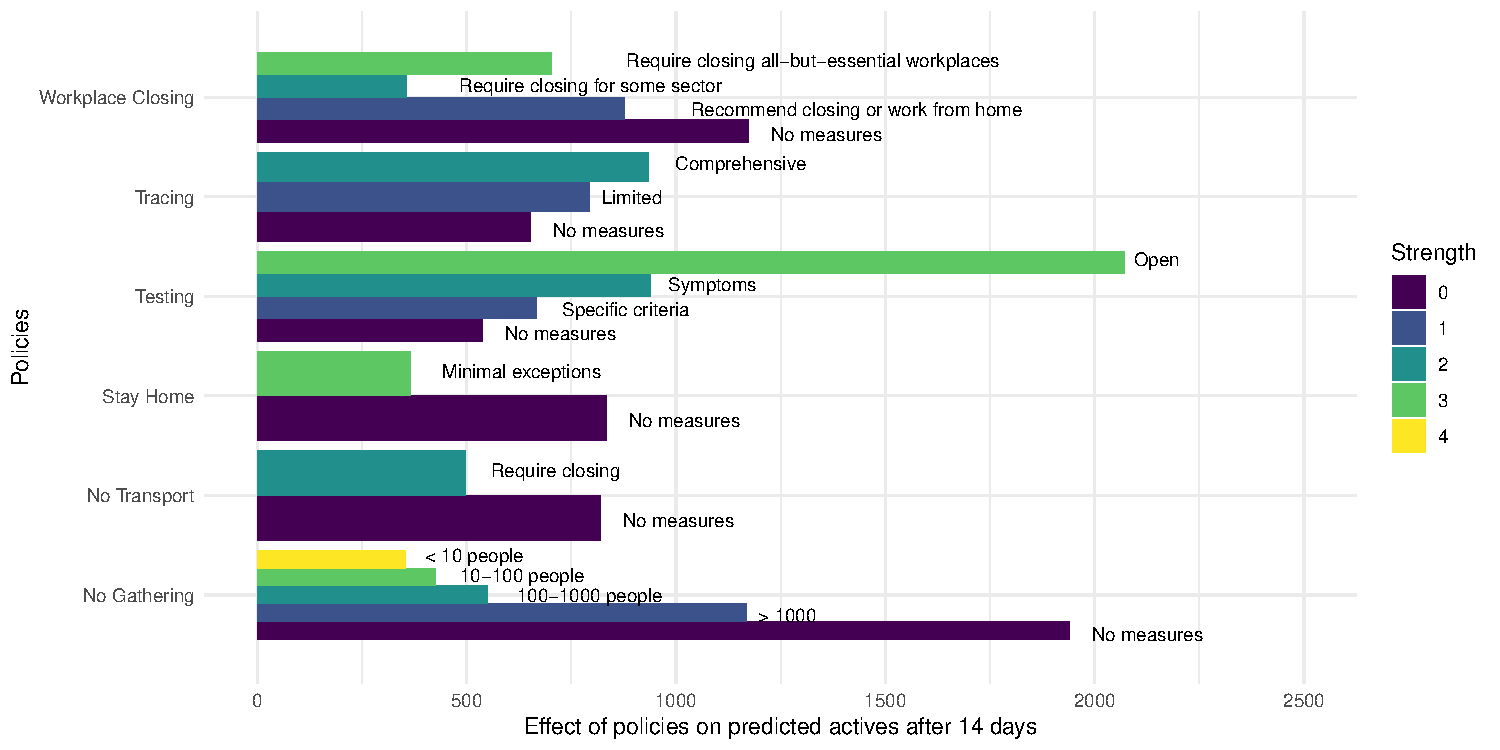
\includegraphics{Report_SC_Group3_files/figure-latex/unnamed-chunk-19-1} \end{center}

We can note that in general, the strong lockdown policies work with
respect to impose no measure. For example, if the government prohibits
most citizens from using public transport, the number of active people
diminishes around \(39.4\%\) with respect to imposing no public
transport measures after \(14\) days when the policy lockdown was
imposed. Also, we can note that weak gatherings restrictions still work
concerning impose no action. For example, restrictions on gatherings
between 100-1000 people diminish the number of active persons around
\(71.62\%\)after \(14\) days when the policy lockdown was imposed.
However, we can see a reverse situation analyzing the effects regarding
the variables describing the testing and tracing policies. Probably,
strong testing and tracing policies lead to discovering more infected
people.

The following plot represents the effects of two policies, i.e.,
workplace closing and gatherings restriction, on predicted active people
\(14\) days after applying these policies.

\begin{center}
	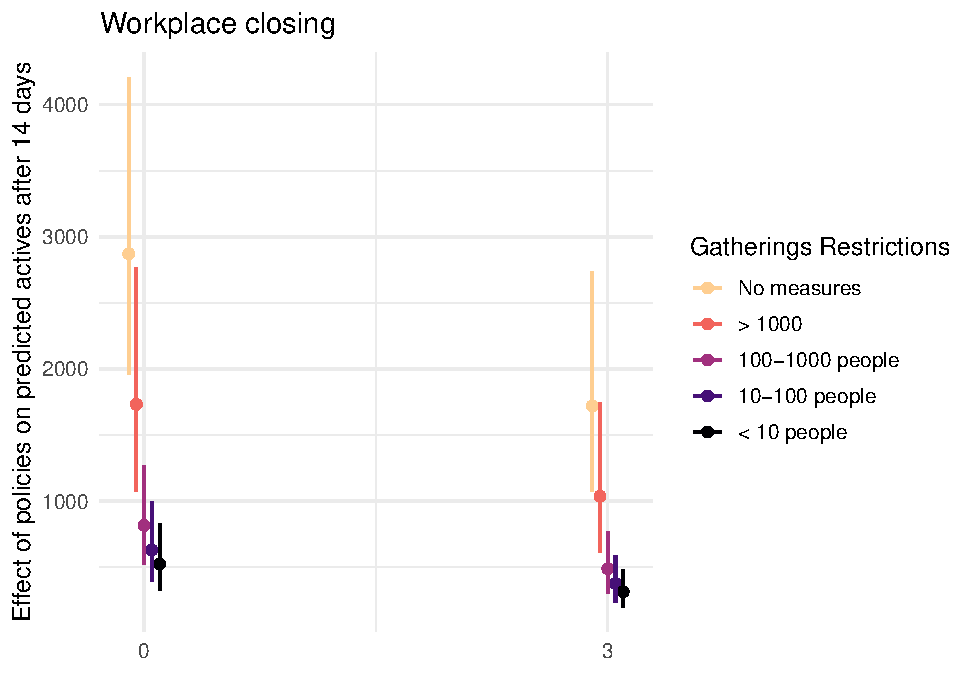
\includegraphics[width=.7\textwidth]{Report_SC_Group3_files/figure-latex/unnamed-chunk-20-1} 
\end{center}

The combination of gatherings restrictions and workplace closing works,
the number of actives decreases, also if the weak limit on reunion is
applied.

\hypertarget{clusters}{%
\subsubsection{CLUSTERS}\label{clusters}}

The following plot represents the effects of the clusters on predicted
actives after \(14\) respect to the cluster associated with Italy.

\begin{center}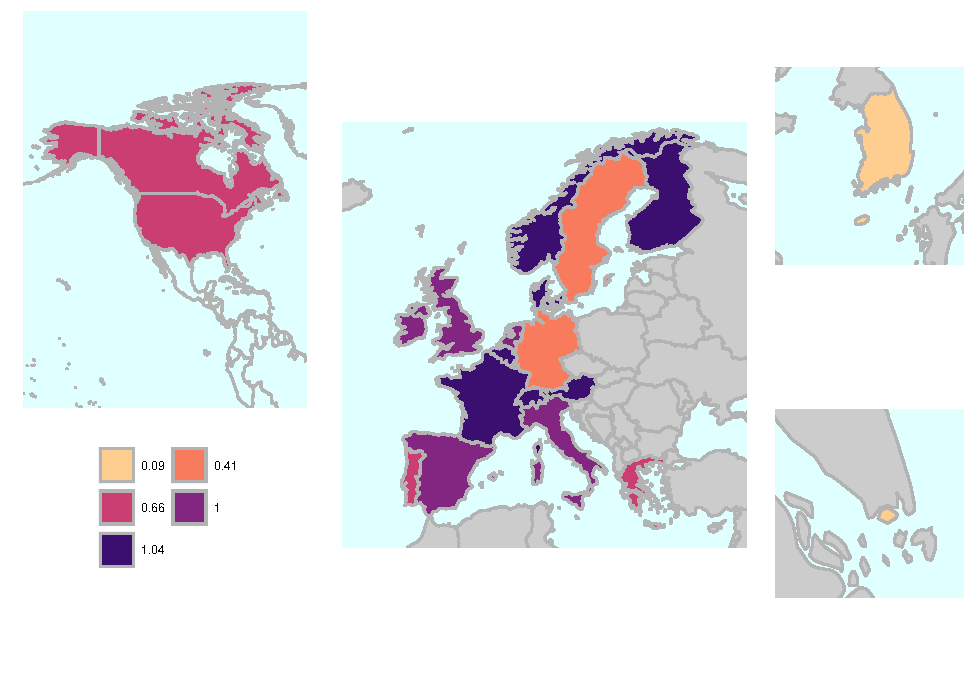
\includegraphics[width=.6\textwidth]{Report_SC_Group3_files/figure-latex/unnamed-chunk-21-1} \end{center}

The following table represents the tests and p-values respect the
countries pairwise comparision adjsted by Tukey's pvalues multiple
comparison procedure adjustment.

\begin{longtable}[]{@{}lrrr@{}}
\toprule
& Std & Test & Pvalues\tabularnewline
\midrule
\endhead
Cl2 - Cl1 & 0.173 & 8.454 & 0.0000000\tabularnewline
Cl3 - Cl1 & 0.158 & 12.377 & 0.0000000\tabularnewline
Cl4 - Cl1 & 0.148 & 16.029 & 0.0000000\tabularnewline
Cl5 - Cl1 & 0.159 & 15.122 & 0.0000000\tabularnewline
Cl3 - Cl2 & 0.137 & 3.607 & 0.0026762\tabularnewline
Cl4 - Cl2 & 0.125 & 7.243 & 0.0000000\tabularnewline
Cl5 - Cl2 & 0.124 & 7.607 & 0.0000000\tabularnewline
Cl4 - Cl3 & 0.106 & 3.870 & 0.0009438\tabularnewline
Cl5 - Cl3 & 0.084 & 5.315 & 0.0000010\tabularnewline
Cl5 - Cl4 & 0.090 & 0.425 & 0.9926511\tabularnewline
\bottomrule
\end{longtable}

We can see that Korea and Singapore are the best countries that acted
appropriately, while Sweden, Germany, Portugal, and Greece are better
than the other European countries. Finally, the USA and Canada are
better than the other European countries except for Sweden and Germany.

\hypertarget{interaction-lockdown-policies-and-clusters}{%
\subsubsection{INTERACTION LOCKDOWN POLICIES AND
CLUSTERS}\label{interaction-lockdown-policies-and-clusters}}

In this Section, the effects of the interaction between each significant
lockdown policy and clusters are examined.

\begin{enumerate}
\def\labelenumi{\arabic{enumi}.}
\tightlist
\item
  Testing policies
\end{enumerate}
\begin{center}
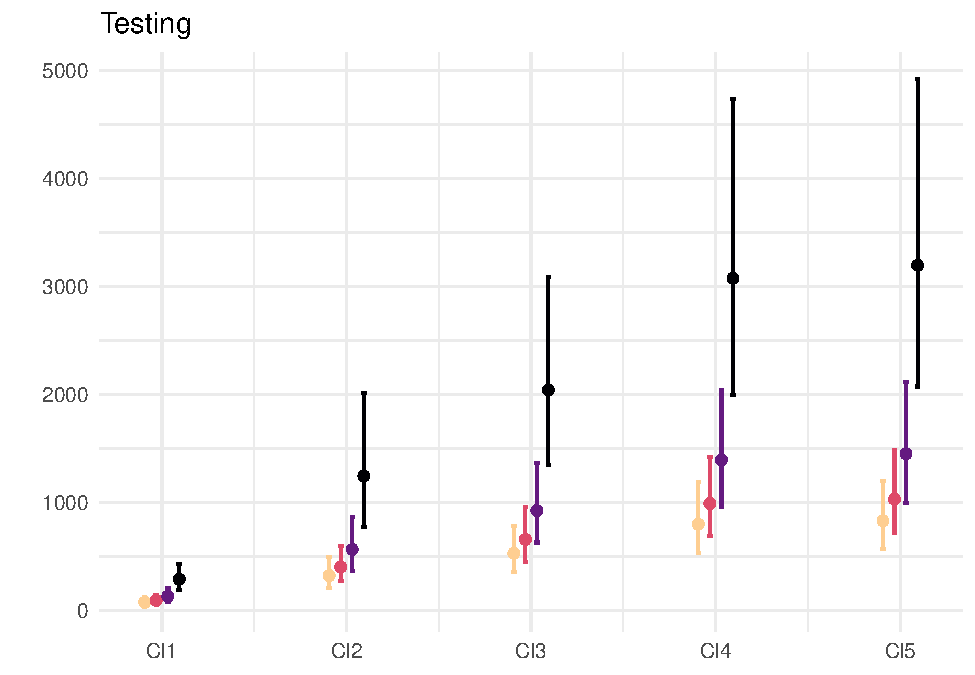
\includegraphics[width=0.7\linewidth]{Report_SC_Group3_files/figure-latex/unnamed-chunk-23-1}
\end{center}
\begin{enumerate}
\def\labelenumi{\arabic{enumi}.}
\setcounter{enumi}{1}
\tightlist
\item
  Contact Tracing
\end{enumerate}
\begin{center}
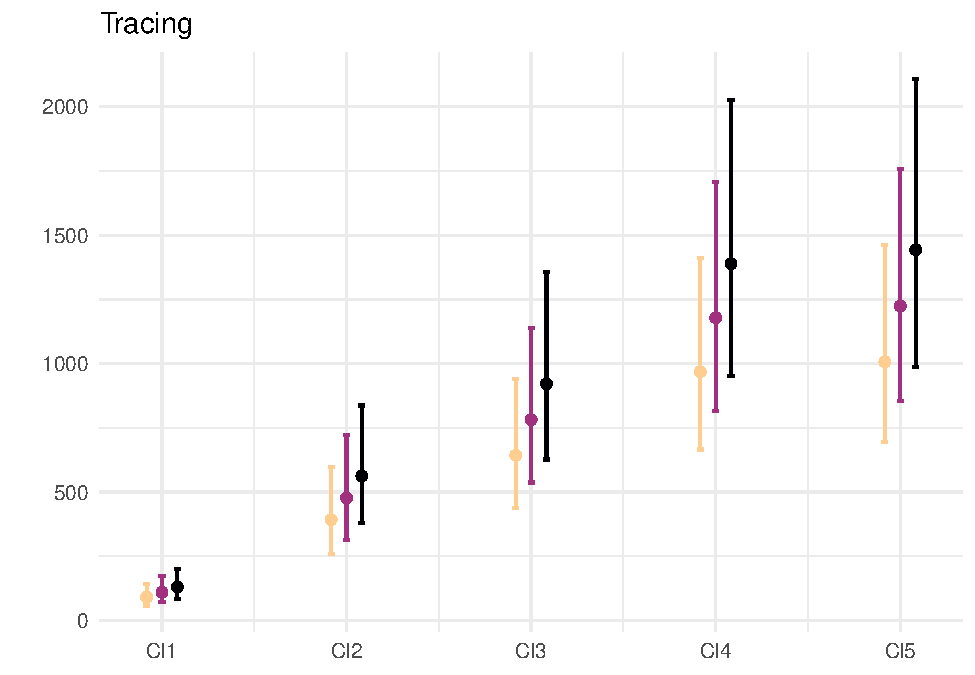
\includegraphics[width=0.7\linewidth]{Report_SC_Group3_files/figure-latex/unnamed-chunk-24-1}
\end{center}
\begin{enumerate}
\def\labelenumi{\arabic{enumi}.}
\setcounter{enumi}{2}
\tightlist
\item
  Gatherings Restrictions
\end{enumerate}
\begin{center}
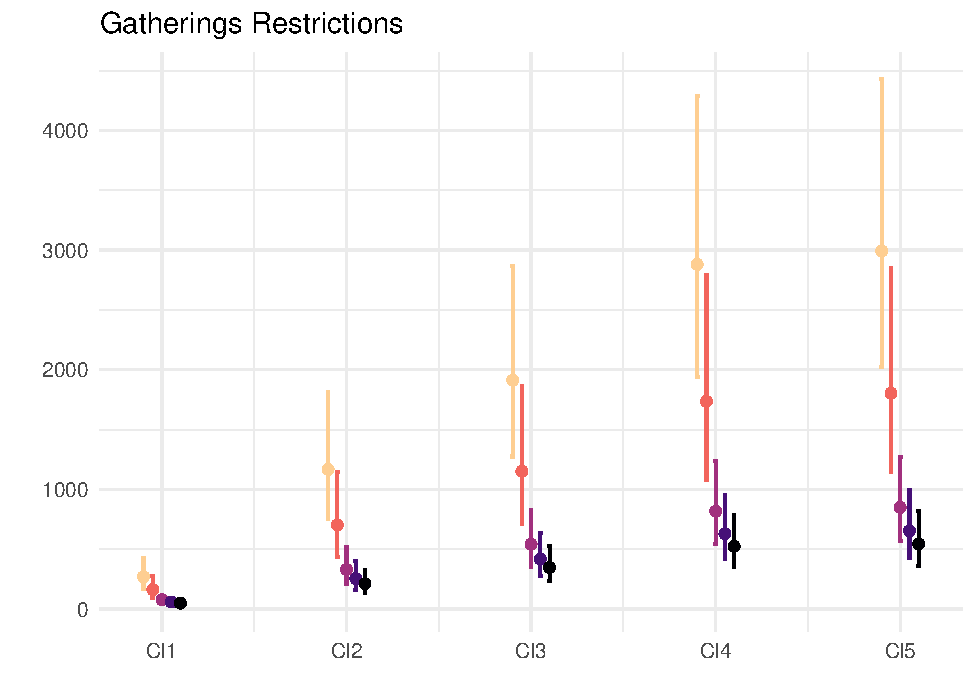
\includegraphics[width=0.7\linewidth]{Report_SC_Group3_files/figure-latex/unnamed-chunk-25-1}
\end{center}
\begin{enumerate}
\def\labelenumi{\arabic{enumi}.}
\setcounter{enumi}{3}
\tightlist
\item
  Stay Home Restrictions
\end{enumerate}
\begin{center}
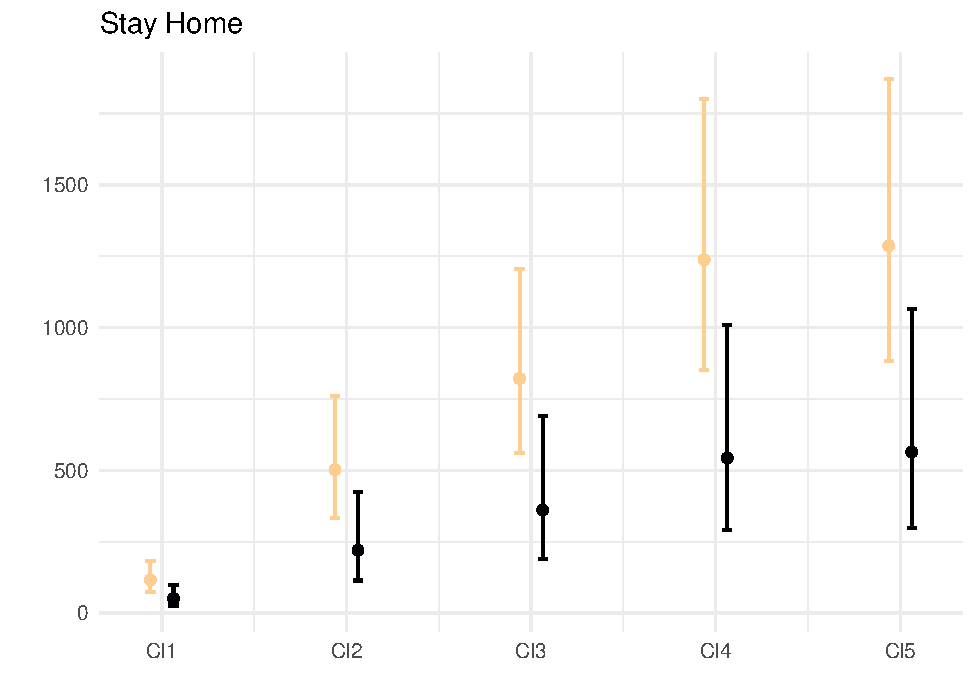
\includegraphics[width=0.7\linewidth]{Report_SC_Group3_files/figure-latex/unnamed-chunk-26-1}
\end{center}
\begin{enumerate}
\def\labelenumi{\arabic{enumi}.}
\setcounter{enumi}{4}
\tightlist
\item
  Workplace Closing
\end{enumerate}
\begin{center}
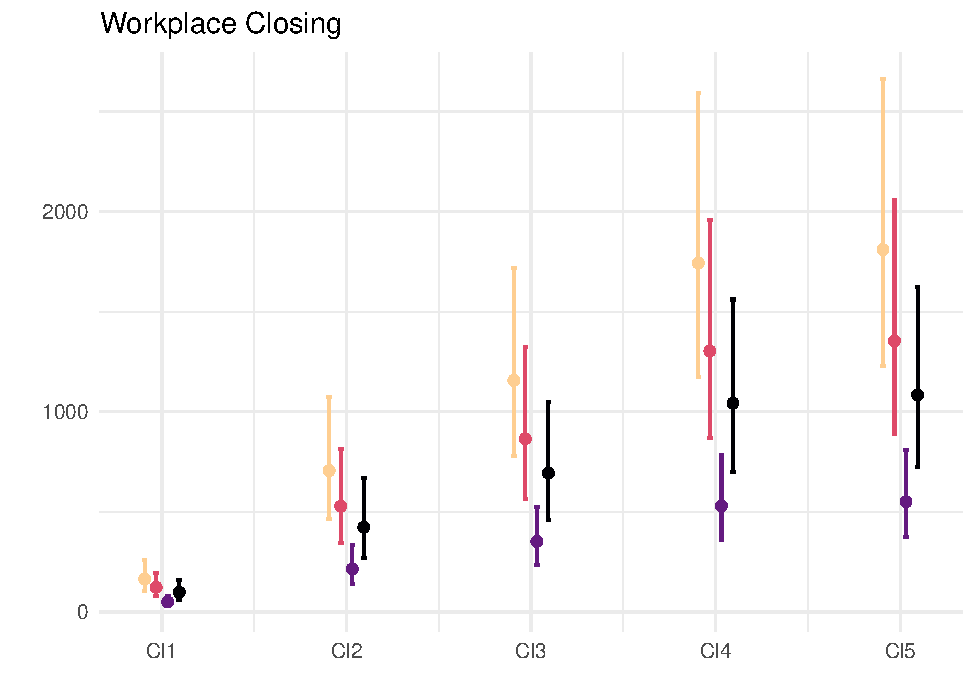
\includegraphics[width=0.7\linewidth]{Report_SC_Group3_files/figure-latex/unnamed-chunk-27-1}
\end{center}
\begin{enumerate}
\def\labelenumi{\arabic{enumi}.}
\setcounter{enumi}{5}
\tightlist
\item
  Transport Closing
\end{enumerate}
\begin{center}
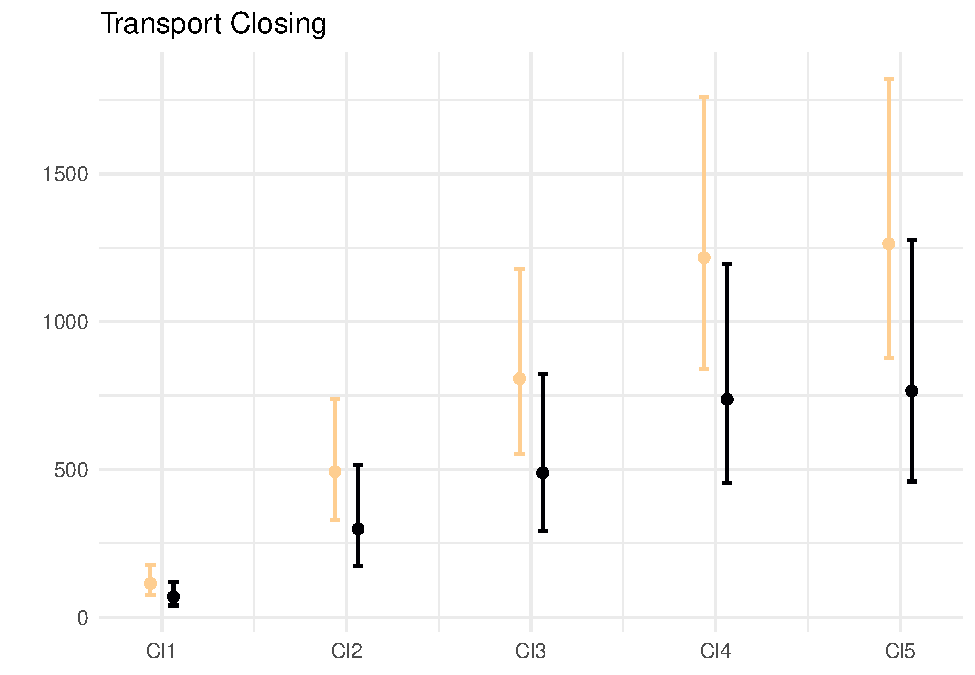
\includegraphics[width=0.7\linewidth]{Report_SC_Group3_files/figure-latex/unnamed-chunk-28-1}
\end{center}
\hypertarget{countries}{%
\subsubsection{COUNTRIES}\label{countries}}

In this Section, the countries' effects on the number of active people
are analyzed, considering \(4\) type of scenarios:

\begin{enumerate}
\def\labelenumi{\arabic{enumi}.}
\item
  \textbf{No measures} of lockdown, tracing and testing policies;
\item
  \textbf{Maximum restriction} of lockdown, tracing and testing
  policies;
\item
  Only maximum level of \textbf{contact tracing and testing policies};
\item
  Only maximum restriction of \textbf{lockdown/social distancing
  policies}.
\end{enumerate}

The effects are computed considering \(100\) and \(1000\) active people
at time \(t\), when the policies are applied. The other covariates are
fixed and equal to the mean value.

\begin{center}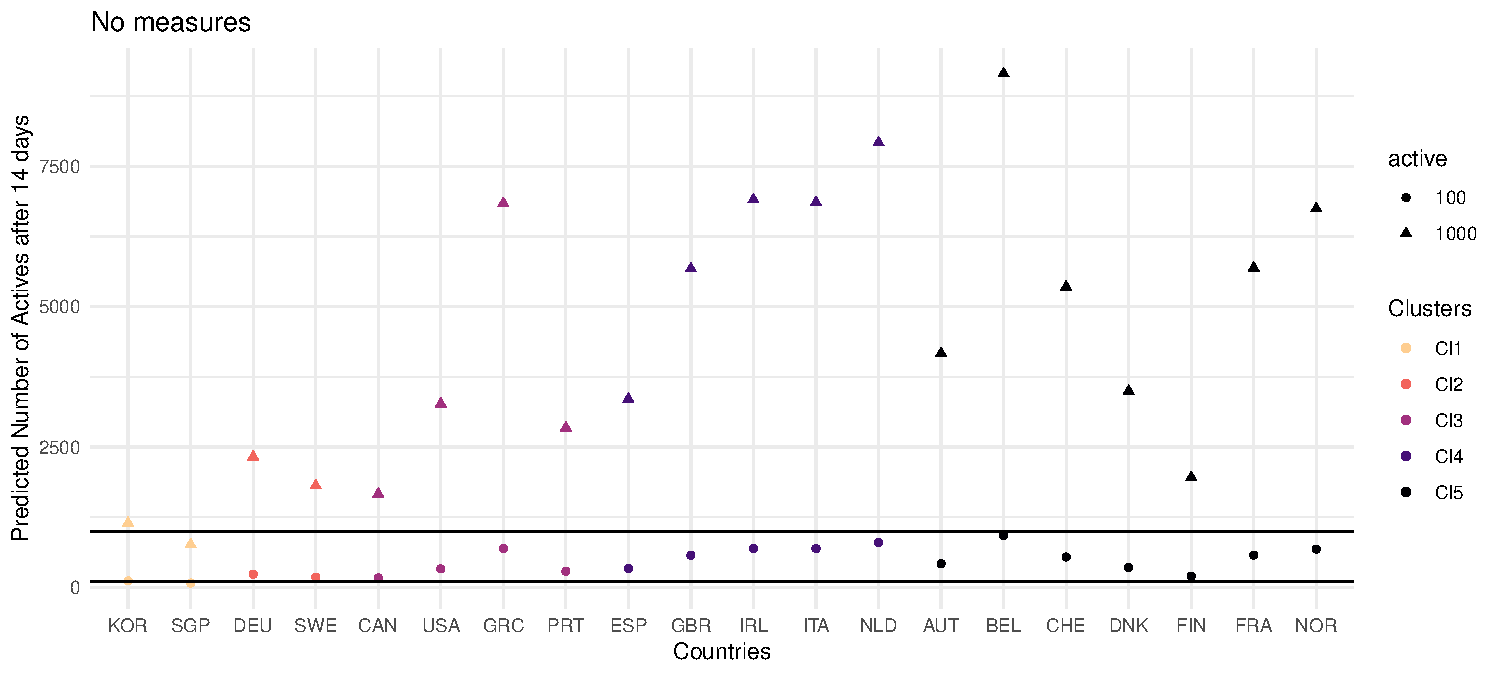
\includegraphics{Report_SC_Group3_files/figure-latex/unnamed-chunk-29-1} \end{center}

If the government doesn't impose any measure to contrast the
coronavirus, the number of active people after \(14\) days will
increase, in particular in the fourth cluster, i.e., Spain, Italy,
Irland, United Kingdom, and the Netherlands. The situation gets worst if
the number of active people at time \(t\) is large.

\begin{center}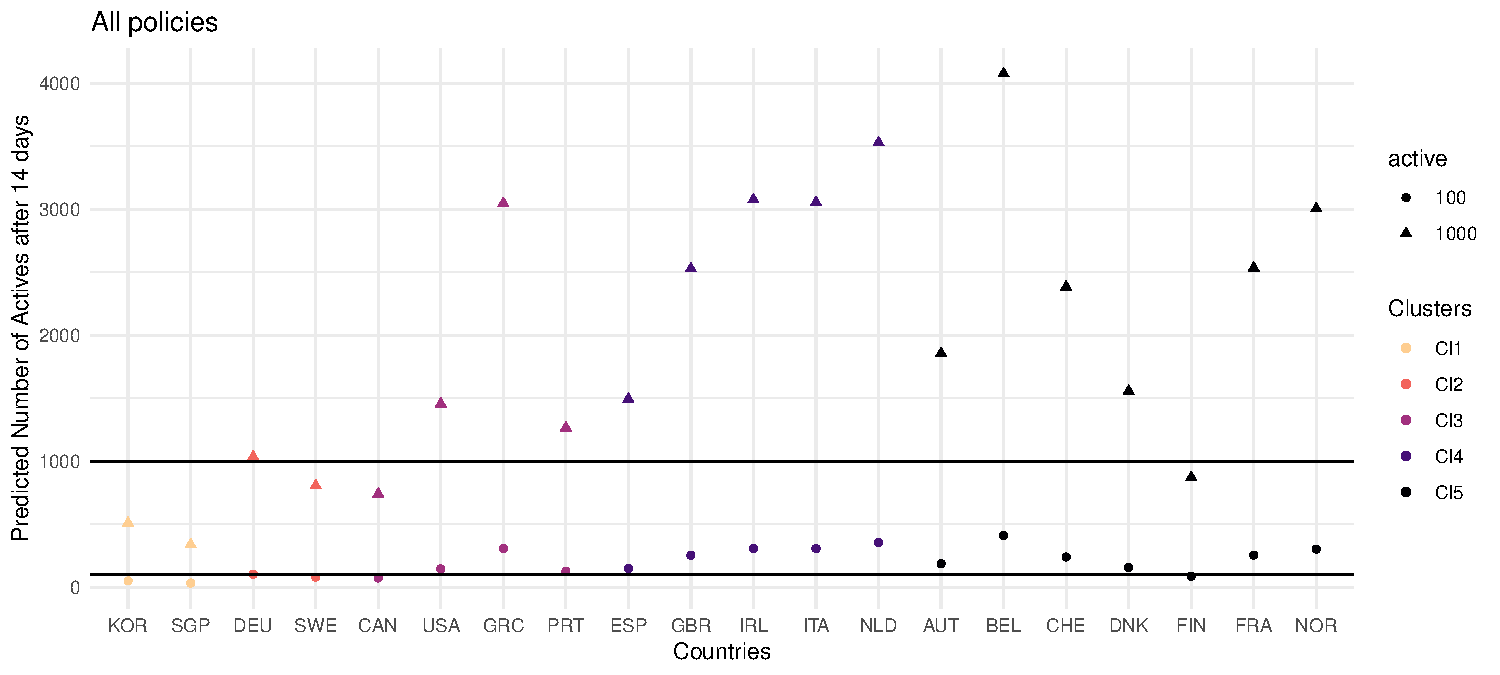
\includegraphics{Report_SC_Group3_files/figure-latex/unnamed-chunk-30-1} \end{center}

The situation gets better if the government applied the strong level of
restrictions about social distancing and the strong levels of testing
and tracing policies. However, the increasing of the number of active
people due to testing and tracing policies influences the analysis of
the effects, as you can see in the following plot:

\begin{center}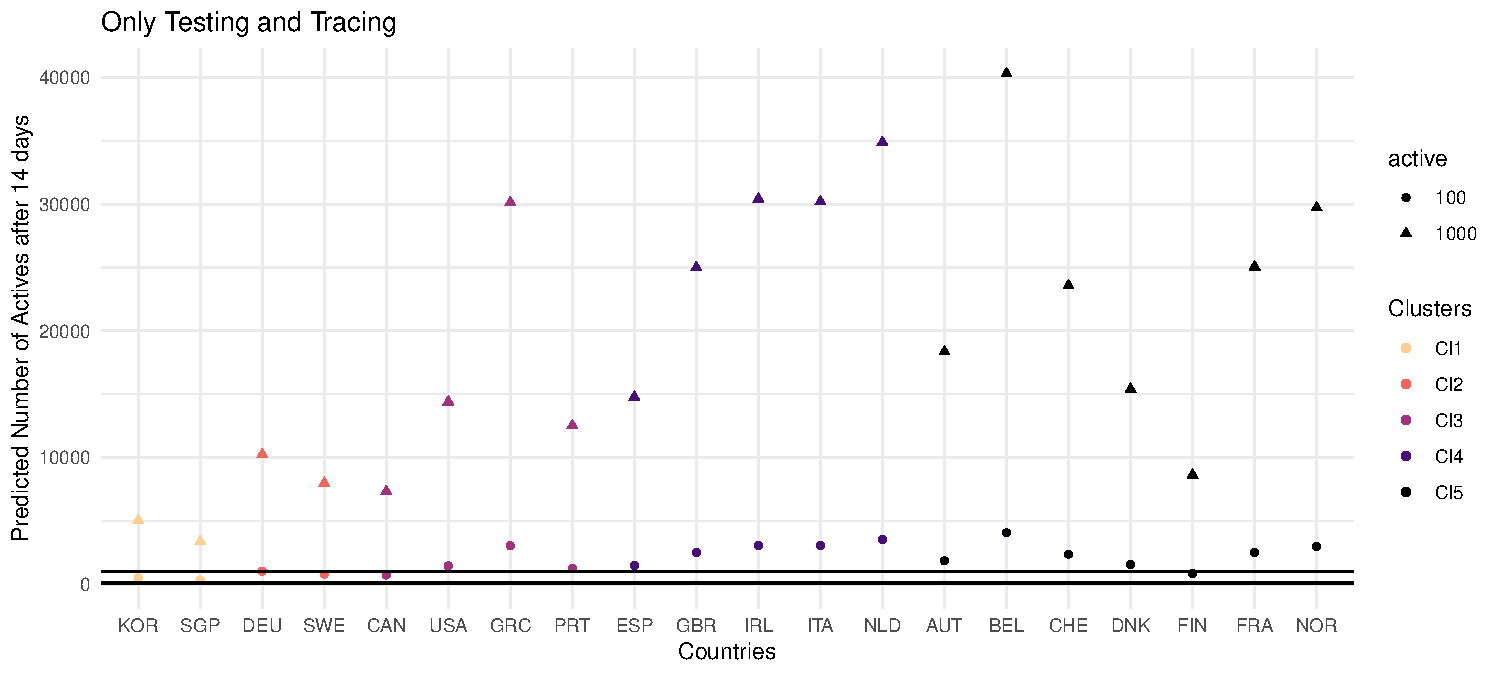
\includegraphics{Report_SC_Group3_files/figure-latex/unnamed-chunk-31-1} \end{center}

The best situation, as expected is the follows:

\begin{center}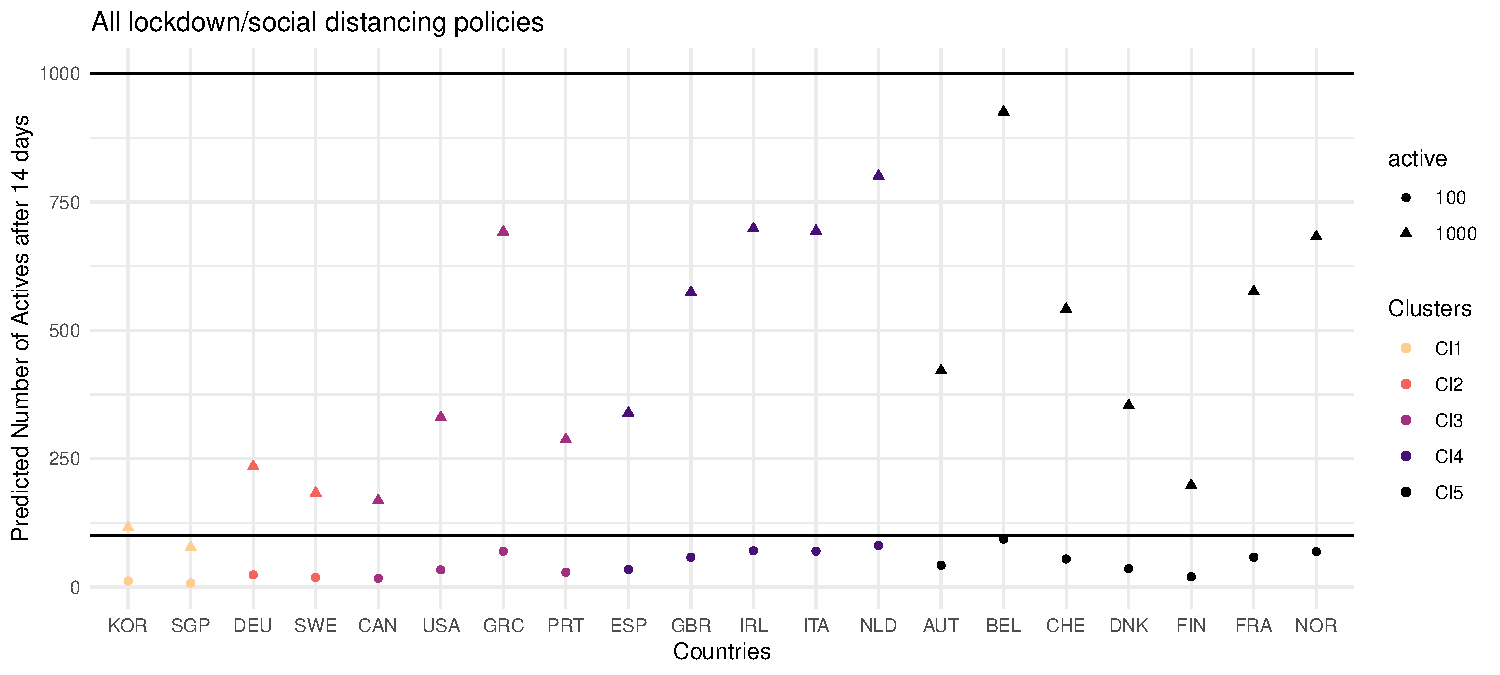
\includegraphics{Report_SC_Group3_files/figure-latex/unnamed-chunk-32-1} \end{center}

i.e., the governements apply the strong levels of all lockdown policies,
in this case the testing and tracing variables are imposed to \(0\).

\hypertarget{to-sum-up}{%
\subsection{To sum up}\label{to-sum-up}}

\begin{enumerate}
\def\labelenumi{\arabic{enumi}.}
\item
  Lockdown policies work with respect to impose no measure in general;
\item
  Weak gatherings restrictions still work, i.e., restrictions on
  gatherings between 100-1000 people;
\item
  Strong Testing and Tracing policies lead to discovering more infected
  people;
\item
  Korea and Singapore are the best countries that acted properly;
\item
  Sweden, Germany, Portugal, and Greece better than the other UE
  countries;
\item
  The USA, and Canada better than the other UE countries except for
  Sweden and Germany.
\end{enumerate}

\hypertarget{italian-lockdown-and-regional-outcomes}{%
\section{Italian lockdown and regional
outcomes}\label{italian-lockdown-and-regional-outcomes}}

In the previous sections, the effect of lockdown policies on the spread
of contagion was estimated for each country, but data is available for
some countries at regional level too. The aim in this section is to
check for differences among \textbf{Italian regions}. Such an analysis
is important for our Phase Two, as governors will have more power in
tayloring lockdown measures down to their regions' needs.

Data is still available from the same sources as before. The effect of
different \textbf{policies} has already been estimated, while now
\textbf{only their aggregate effect} can be assessed. Indeed the
countermeasures for COVID19 escalated almost simultaneously all over the
country (excepted the Red Zone, but only for few days) and on all sides
(as to offices, schools, transit, etc). So in this analysis, all
different policies are replaced by a single factor, which is the Phase:
Zero, One. As to the newer Phase Two, too few days of data are
available, so it will be discarded.

Italian regions are known to be separated by a relevant divide under all
socio-economic aspects. Unfortunately, integration among the COVID19 R
package and other databases came lately, and manual linkage with other
sources was hard, so that fewer variables are available at a regional
level. Nonetheless, the mixed- and \textbf{random- effects} approach
exploited in previous sections can still be useful in accounting for all
the unobserved heterogeneity. Random effects can be used to address
several problems, namely: some regions have less resources to find their
infected inhabitants, so that the real proportions of contagion are
bigger than numbers can say in some poorer regions.

The time series of active cases is definitely not smooth, because cases
are often spotted in bulks. Especially in early days of the emergency,
the trend in active cases is highly non-stationary and many smoothing
methods have failed in our analysis, both in the previous national-wise
analysis and in the next regional-wise analysis. In order to best catch
up with the non-stationarity, we adopt an approach that we call
``\textbf{auto-regressive}'', in the sense that we try to predict future
counts of active cases based on the current counts. Predictions in this
case stick less to older values and the model can follow the real trend
more easily. This constitutes a safe control for baseline conditions,
which are known to differ among regions, in that, e.g., the
\textbf{international hubs} Lazio and Lombardia were struck earlier and
more heavily by the Virus.

Stated plainly, we model the relative increase of active cases that one
can expect in 14 days, given the current cases and the causes of
variation, that is, the type of lockdown and demographics of the
regions. As in standard \textbf{panel data approach}, the regions make
up the individuals, on which some measures are repeated on a daily
basis.

One random effect is assigned to \textbf{regions} and one to the
\textbf{day}. This accounts for differences among regions and also for
general changes in testing abilities. Moreover, the random effect for
regions can change between \textbf{phases}. One more random effect is
\textbf{day-and-region} specific, and it accounts for any badness in
data collection or outlying events. It also solves the overdispersion
problem with count data models like Poisson and binomial. As shown
later, this stratagem allows to boil down the effect of testing errors,
as it happened in Friuli and other regions now and then.

The auto-regressive approach has the disadvantage of explaining most of
future outcomes by using previous outcomes, which leave small room for
assessing the effect of several demographic variables, which are
(almost) \textbf{constant} through time. The effect of such demographic
predictors is summed up by the aforementioned random effects though.

One could model the prevalence, or the proportion of active cases over
the population, by means of a binomial model. But we saw that, even
though the actives are not few, an approximation to \textbf{Poisson}
still holds. Binomial and Poisson models were seen to be very similar to
each other, so only the Poisson model is reported. Small changes in the
attached R codes can return both results and are on to the reader.

\hypertarget{results-1}{%
\subsection{Results}\label{results-1}}

The model in use allows to estimate the expected relative variation of
active cases in two weeks. This lag was chosen based on the latency of
COVID19, which is the time we thought one would have to wait before the
effect of any policies could be observed. Prediction intervals based on
the behavior on the last day are reported in the following. The last day
considered comes right after two weeks have elapsed after May 18th's
retail reopenings.

The random effects in use make it difficult to interpret the estimates,
so we provide some summaries in the following to make the implications
of our model more clear.

\begin{center}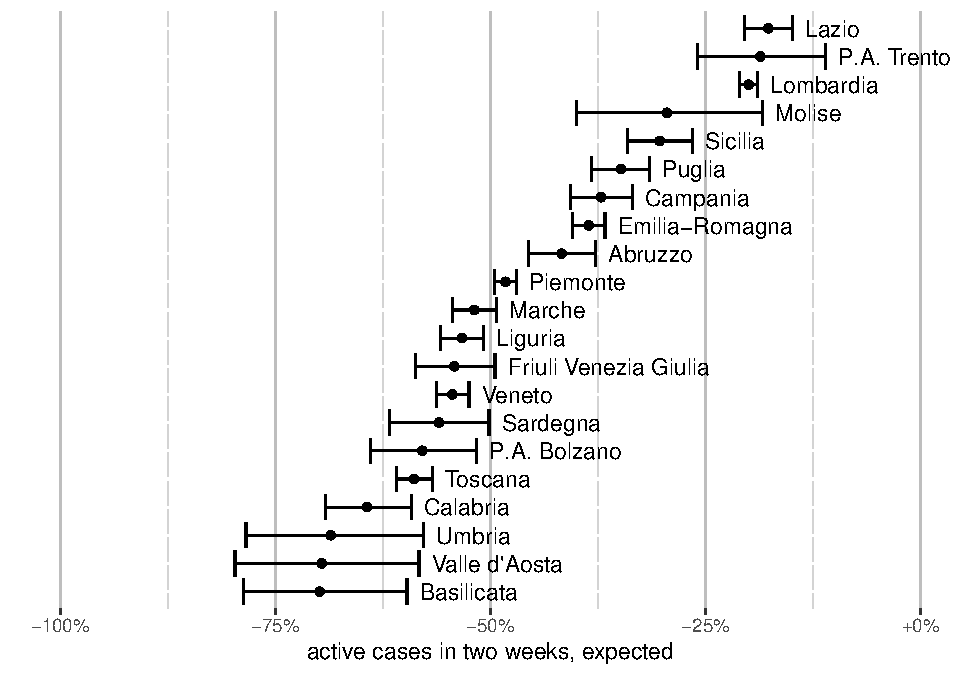
\includegraphics{Report_SC_Group3_files/figure-latex/unnamed-chunk-34-1} \end{center}

One can see that the slowest recovery is observed in Lazio and
Lombardia, which also serve as the Italian international hubs, from both
a political and economic point of view. Larger confidence intervals
correspond to regions that are smaller or hit less by the Virus. The
case of Molise will be seen in the following as a rather peculiar one.

The \textbf{take home message} here is that the international hubs would
be jeopardized in the case of a slightly liberal Phase Two. In their
case, it would be safer to still adopt restrictive measures, while the
other regions may drive the economic recovery, since they have a larger
margin of action, their recovery being faster.

Based on the relative variation of active cases expected in two weeks,
denoted \(RV\), and on the current cases \(I_t\) on day \(t\), one can
roughly estimate the implied cases on day \(s\) with:
\[I_s = I_t \times RV^{(s-t)/14}\,\] which matches the definition of
\(RV\) when \(s-t=14\).

One can think of the Estimated Time to Recovery (ETR, in days) as the
time needed on average for the active cases less than, say, \(n=\) 30.
The ETR is related to the current cases \(I_t\) and the \(RV\) as:
\[n \leq I_t \times RV^{ETR/14} \,,\] which implies the definition
\[ETR/14 = \log(n/I_t)/\log(RV) \,,\] for the estimated weeks to
recovery. When \(RV\) is bigger than one, so the contagion is not under
control, the ETR is negative. In the case of Italian regions, on the
last day considered here, all the regions were, at a reasonable
confidence level of \(95\%\), behaving appropriately, as the \(RV\) is
less than one. In the following, the ETR is reported for each region.

\begin{center}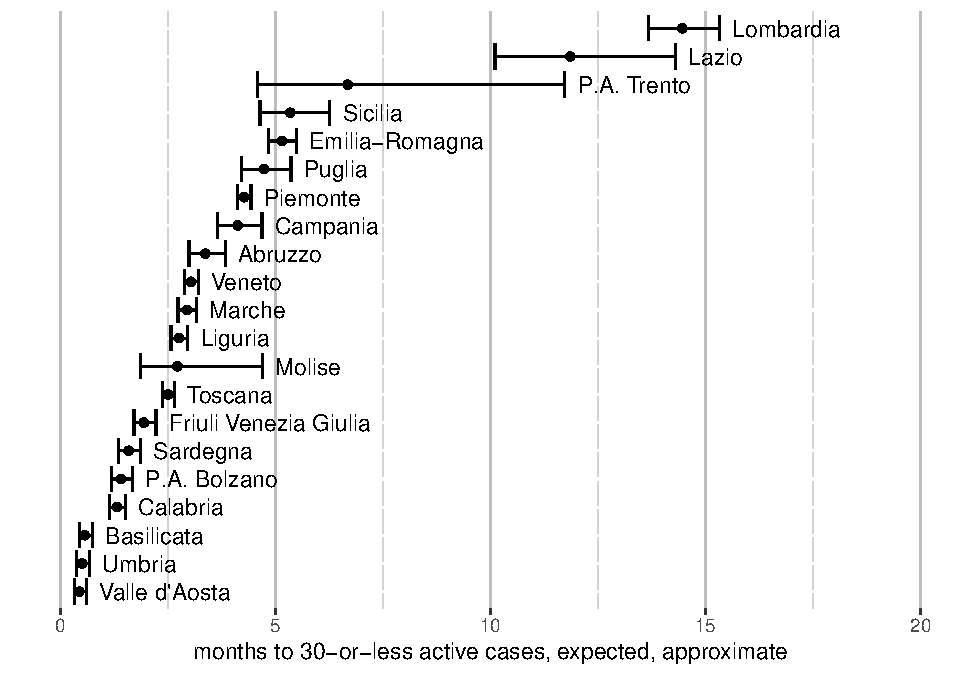
\includegraphics{Report_SC_Group3_files/figure-latex/unnamed-chunk-35-1} \end{center}

As one can see, even by rescaling and considering months- instead of
weeks- to recovery, we are far away from full recovery. In the case of
Lombardia and Lazio, several months are required before they recover in
full. This makes it even more imperative than previously seen to still
enforce some restrictive countermeasures in Lombardia and Lazio, because
even with Phase One-like measures it would take about one year or more
to defeat the Virus.

The two features seen before, the rate of recovery and the time to
recovery, the latter combining the former and the currently active
cases, can be seen one versus the other, as follows.

\begin{center}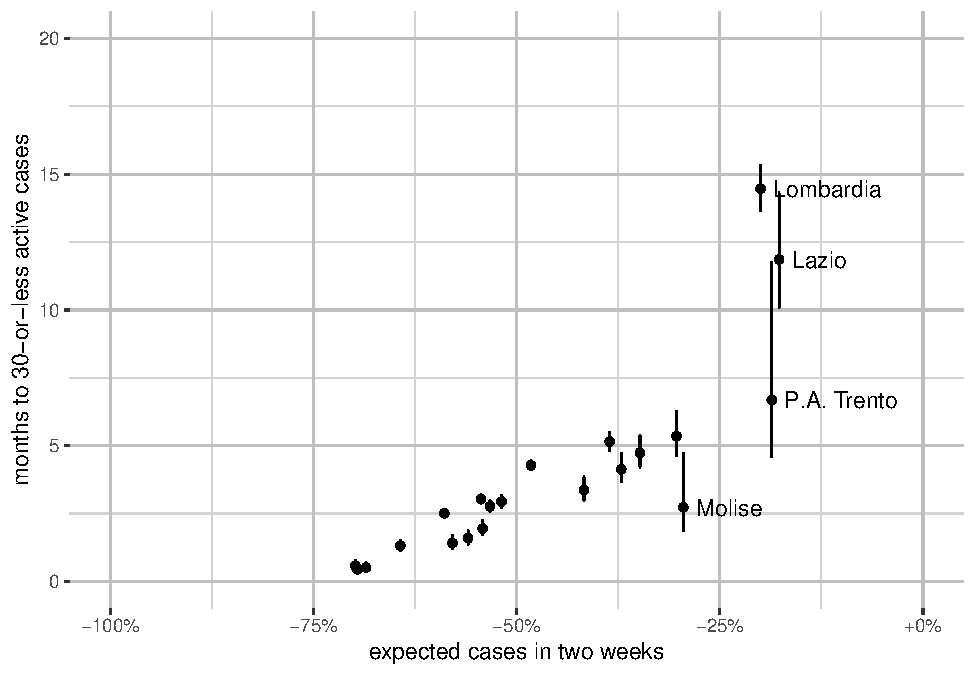
\includegraphics{Report_SC_Group3_files/figure-latex/unnamed-chunk-36-1} \end{center}

Lombardia and Lazio are far out of the trend that seems to link the rate
and time to recovery, as their time to recovery is slightly longer than
that of any region with comparable rate of recovery, which must be due
to the outlying number of current active cases.

We just focus on the rate of recovery, while remembering of the anomaly
represented by the international hubs. So one can see from the following
map that reopenings surgically taylored down to the specific regions may
take place, though it might be required to forbid or restrict travel to
and from those areas.

\begin{center}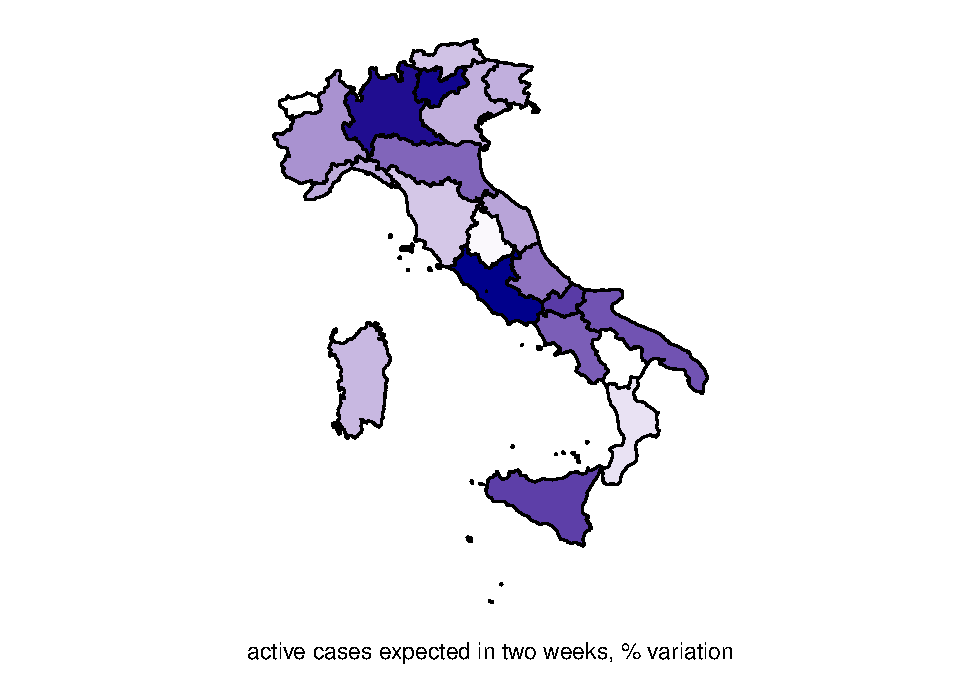
\includegraphics{Report_SC_Group3_files/figure-latex/unnamed-chunk-37-1} \end{center}

Moreover, pressures in favor of reopening might be listened to in some
industrially relevant regions like Veneto. As to holiday destinations,
it is somewhat questionable the extent to which regions like Basilicata
and Calabria might have performed their testings and lockdown
enforcement. To our knowledge, the quality of data related to these two
regions was already discussed by another team.

Overall, our regions have achieved a good level of contagion
containment, by working it out week after week as testified by the
following plot. The predicted rate of recovery is plotted on daily
basis. This works as a Poisson model-based smoothing of the rate of
change in active cases. As one can see, many regions had the epidemic
out of control for a rather long time, but the prompt response of the
most affected regions has driven the contagion down to compensate for
late responses anywhere else.

\begin{center}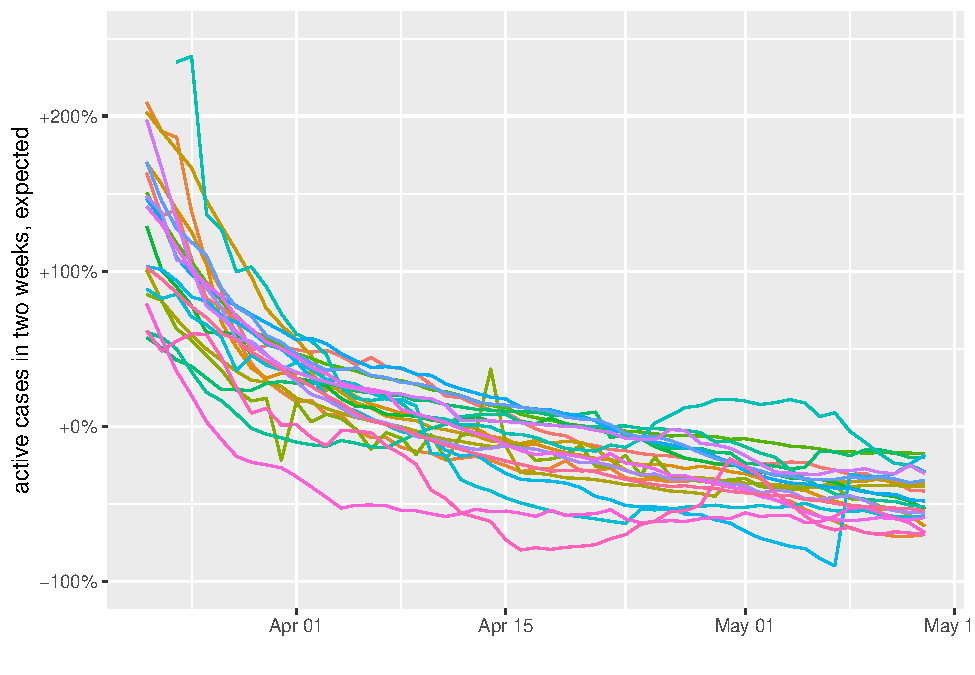
\includegraphics[width=0.7\linewidth]{Report_SC_Group3_files/figure-latex/unnamed-chunk-38-1} \end{center}

Irregularities in the trend that catch one's attention may be,
primarily:

\begin{itemize}
\tightlist
\item
  mis-counts of cases in Friuli around half-April, as reported by guests
  at the seminar before the report,
\item
  prolonging emergency in Molise,
\item
  overall good behavior of Umbria and Valle d'Aosta, worsening quite
  abruptly and steadily ever after some point in Trentino.
\end{itemize}

The estimated trend in Phase Zero is just too unstable to deserve
reporting here. One must consider though that, compatibly with the
results from previous sections on countries data, the epidemic was
unquestionably out of control before the lockdown, and that the
epidemics is still on the verge of booming again across Italy even under
Phase One-like measures. This mandates for cautious and restrictive
approaches from every region.

\hypertarget{to-sum-up-1}{%
\subsection{To sum up}\label{to-sum-up-1}}

\begin{enumerate}
\def\labelenumi{\arabic{enumi}.}
\item
  The epidemic curve is currently under control in all Italian regions.
\item
  The case of economic and political hubs, Lombardia and Lazio, is just
  peculiar, with slow recovery and worst baseline conditions. In all
  other regions, the epidemic is expected to end soon.
\item
  Lombardia and Lazio might have to wait at least one year before the
  active cases fall far below the hundreds units. The other regions
  could drive the economic recovery in the meantime.
\item
  The margin of action to de-escalate lockdown policies, though, is
  limited. The example provided by Korea and Singapore on contact
  tracing and testing might be followed closely, after the successes
  highlighted in the previous sections.
\end{enumerate}

\hypertarget{supplementary-materials}{%
\section{Supplementary materials}\label{supplementary-materials}}

All the codes used for this analysis are available on
\href{https://github.com/angeella/Lockdown_policies_COVID19}{Github}.
The report was written by rmarkdown, fully reproducible. You can find
the rmarkdown file in
\href{https://github.com/angeella/Lockdown_policies_COVID19/Report}{Github}.

\hypertarget{references}{%
\section*{References}\label{references}}
\addcontentsline{toc}{section}{References}

\hypertarget{refs}{}
\begin{cslreferences}
\leavevmode\hypertarget{ref-funfem}{}%
Bouveyron, Charles, and Julien Jacques. 2015. ``FunFEM: An R Package for
Functional Data Clustering.'' In \emph{Quatrième Rencontres R}.

\leavevmode\hypertarget{ref-glmmTMB}{}%
Brooks, M. E., K. Kristensen, K. J. van Benthem, A. Magnusson, C. W.
Berg, A. Nielsen, H. J. Skaug, M. Mächler, and B. Bolker. 2017.
``GlmmTMB Balances Speed and Flexibility Among Packages for
Zero-Inflated Generalized Linear Mixed Modeling.'' \emph{The R Journal}
9 (2): 378--400.

\leavevmode\hypertarget{ref-Jhon}{}%
Dong, E., H. Du, and L. Gardner. 2020. ``An Interactive Web-Based
Dashboard to Track Covid-19 in Real Time.'' \emph{Lancet Infect Dis}.

\leavevmode\hypertarget{ref-Hardin}{}%
Hardin, J. W., and J. M. Hilbe. 2018. \emph{Generalized Linear Models
and Extensions}. 4th ed. Stata Press.

\leavevmode\hypertarget{ref-Nakagawa}{}%
Nakagawa, S., and H. Schielzeth. 2013. ``A General and Simple Method for
Obtaining \(R^2\) from Generalized Linear Mixed‐effects Models.''
\emph{Methods in Ecology and Evolution} 4 (2): 133--42.

\leavevmode\hypertarget{ref-Oxford}{}%
Thomas, H., S. Webster, A. Petherick, T. Phillips, and B. Kira. 2020.
``Oxford Covid-19 Government Response Tracker, Blavatnik School of
Government.'' \emph{Data Use Policy: Creative Commons Attribution CC BY
Standard}.
\end{cslreferences}

\end{document}
